\documentclass[a4paper,11pt]{article}
% \pdfoutput=1 % if your are submitting a pdflatex (i.e. if you have
             % images in pdf, png or jpg format)
\usepackage{jcappub} % for details on the use of the package, please
                     % see the JCAP-author-manual
\usepackage[T1]{fontenc} % if needed
\usepackage{float} 
\usepackage{lmodern}
\usepackage{booktabs}
\usepackage{siunitx}
\usepackage[english]{babel}
\addto\captionsenglish{
  \renewcommand{\figurename}{Figure}
  \renewcommand{\tablename}{Table}
}
\usepackage[utf8]{inputenc}
\usepackage{natbib}
\usepackage[colorlinks=true, citecolor=blue, urlcolor=blue, linkcolor=blue]{hyperref} 
\usepackage{graphicx}
\usepackage{subfigure}% Include figure files
\usepackage[justification=raggedright]{caption}
\usepackage{tabularx}
\usepackage{dcolumn}% Align table columns on decimal point
\usepackage{bm}
% \usepackage{ulem}

\newcommand{\ms}{M_\odot}
\newcommand{\bmt}{{\bm{\theta}}}
\newcommand{\bmT}{{\bm{\Theta}}}
\newcommand{\bmH}{{\bm{H}}}
\newcommand{\rmd}{{\rm{d}}}
\newcommand{\ZW}[1]{\textcolor{magenta}{$\mathcal{ZW}$:~#1}}

% \newcommand{\DL}[1]{\textcolor{red}{#1}} 
% \newcommand{\LS}[1]{\textcolor{cyan}{\bf #1}} 
% \newcommand{\YG}[1]{\textcolor{blue}{#1}} 
% \newcommand{\ZW}[2]{{\color{blue} \sout{#1} ZW: {#2}}} % For comment
% \newcommand{\Reply}[1]{{\bf\color{blue} #1}}

\title{Inference of Love-Q relations with gravitational waves in hierarchical Bayesian framework}

%% %simple case: 2 authors, same institution
%% \author{A. Uthor}
%% \author{and A. Nother Author}
%% \affiliation{Institution,\\Address, Country}

% more complex case: 4 authors, 3 institutions, 2 footnotes
\author[a]{Zhihao Zheng,}
\author[b,c,1]{Ziming Wang\note{Corresponding author.},}
\author[d]{Jinwen Deng,}
\author[b,c]{Yiming Dong,}
\author[c,e,1]{and Lijing Shao}


% The "\note" macro will give a warning: "Ignoring empty anchor\cdots"
% you can safely ignore it.

\affiliation[a]{School of Yuanpei, Peking University,
Beijing 100871, China}
\affiliation[b]{Department of Astronomy, School of Physics, Peking University,
Beijing 100871, China}
\affiliation[c]{Kavli Institute for Astronomy and Astrophysics, Peking
University, Beijing 100871, China}
\affiliation[d]{School of Physics, Peking University,
Beijing 100871, China}
\affiliation[e]{National Astronomical Observatories, Chinese Academy of
Sciences, Beijing 100012, China}

% \affiliation[a]{One University,\\some-street, Country}
% \affiliation[b]{Another University,\\different-address, Country}
% \affiliation[c]{A School for Advanced Studies,\\some-location, Country}

% e-mail addresses: one for each author, in the same order as the authors
\emailAdd{2300017794@stu.pku.edu.cn}
\emailAdd{zwang@pku.edu.cn}
\emailAdd{2300011335@stu.pku.edu.cn}
\emailAdd{ydong@pku.edu.cn}
\emailAdd{lshao@pku.edu.cn}

\abstract{Nuclear and gravity theories have predicted a universal ``Love-Q'' 
relation between the dimensionless tidal deformability $\Lambda$ and the 
dimensionless quadrupole moment $Q$ of neutron stars (NSs). However, this Love-Q 
relation has not yet been directly measured in an observational aspect. 
Gravitational waves (GWs) emitted from binary NS systems serve as 
a powerful tool for probing NS properties. The future next-generation 
GW detectors are expected to yield numerous BNS events with high-precision  
measurements. In this study, we explore the prospects of constraining the Love-Q 
relation with future GW observations. Adopting a hierarchical Bayesian framework, 
we are able to combine multiple GW events in a more systematic manner. 
We simulate 1000 GW sources and select the loudest 20 events for the analysis.
By considering four polynomial models from linear to quartic terms, we find that 
a linear relation 
between $\ln\Lambda$ and $\ln Q$ is accurate enough in constraining the Love-Q
    relation with GWs.
Strong correlations between the parameters are found in all four models. 
Furthermore, we utilize the inferred Love-Q relation in testing modified gravity. Taking the dynamical Chern-Simons gravity as an example, 
our results suggest that the characteristic length $\xi_{CS}^{1/4}$ can be limited 
to about $10\, \mathrm{km}$ or less with future GW observations. 
}

\begin{document}
\maketitle
\flushbottom

%=============================
\section{Introduction}
\label{sec:introducion}
%=============================

Neutron stars (NSs) serve as natural laboratories for studying nuclear and 
gravitational physics due to their extreme densities and strong gravitational 
fields. Electromagnetic observations of NSs, such as their observed maximum 
mass~\cite{Ozel:2010bz,Hebeler:2013nza,Antoniadis:2013pzd} and mass-radius 
relation~\cite{Lattimer:2006xb,Steiner:2010fz,Ozel:2010fw,Özel_2013,Guver:2013xa}, 
allow one to probe the properties of nuclear matter at densities exceeding nuclear 
saturation density. Additionally, the recent observation of GW170817 has opened up a 
new observational window for investigating NS properties using gravitational waves 
(GWs) emitted during binary NS (BNS) coalescences~\cite{LIGOScientific:2017vwq,LIGOScientific:2018cki,
LIGOScientific:2018hze}. Some of NS properties, including the tidal
deformability and the
spin-induced quadrupole moment, contribute to the GW emission
~\cite{Poisson:1997ha,
Vines:2011ud,Favata:2013rwa,Wade:2014vqa,Samajdar:2019ulq,Abac:2023ujg} and 
therefore can be measured from GW observations~\cite{Harry:2018hke,
Baiotti:2019sew,Chatziioannou:2020pqz,Agathos:2015uaa,Krishnendu:2017shb,Krishnendu:2019tjp,Lyu:2023zxv}. 

In a BNS system, each NS is deformed due to the gravitational field of its
companion, leading to an induced mass quadrupole moment
~\cite{Hinderer:2007mb,Damour:2009vw}. The effect is 
characterized by the tidal deformability $\Lambda=2k_2/(3C^5)$, where $k_2$ is the 
tidal Love number and $C$ is the NS compactness~\cite{Flanagan:2007ix}. Also, a 
rotating NS experiences another deformation due to its spin, which induces another
quadrupole moment $\mathcal{Q}=-Q\chi^2 m^3$, called the spin-induced quadrupole
moment, where $Q$ is the dimensionless quadrupole moment, $\chi$ and $m$ are 
the dimensionless spin and mass of the NS respectively~\cite{Hartle:1968,Laarakkers:1997hb}. 
Both $\Lambda$ and $Q$ are determined by $m$
 with a given equation of state 
(EOS)~\cite{Yagi:2013awa}, which describes the relation between pressure and
density of the NS.

On the one hand, the EOS of NSs have not yet been determined by current
observations. On the
other hand, Yagi 
and Yunes~\cite{Yagi:2013bca,Yagi:2013awa} proposed a universal relation between 
$\Lambda$ (or tidal Love number) and $Q$, which is EOS-insensitive 
with variation of about $1\%$ or less for different EOSs in general relativity (GR).
However, this relation is dependent on the underlying gravity theory and thus
provides a powerful approach to testing gravity while avoiding the uncertainties
from the unknown EOS~\cite{Yagi:2013bca,Silva:2020acr,Shao:2022koz}. If the Love-Q relation in GR is adopted as a prior in the waveform
model, the number of independent parameters can be reduced, which helps to
better estimate the spin parameters of BNSs~\cite{Yagi:2013bca,LIGOScientific:2018cki,
LIGOScientific:2018hze,LIGOScientific:2020aai}. 

Future next-generation (XG) ground-based GW detectors, including the Cosmic Explorer 
(CE)~\cite{Reitze:2019iox,Reitze:2019dyk} and the Einstein Telescope (ET)~\cite{Punturo:2010zz,Hild:2010id,Sathyaprakash:2012jk}, 
are expected to
 detect much more GW signals, up to about $10^5$--$10^6$ events per year
~\cite{LIGOScientific:2017zlf,Sathyaprakash:2019yqt,Kalogera:2021bya,Samajdar:2021egv}, 
thanks to their 
increased sensitivity and lower cutoff frequencies. These high-precision GW observations allow us to treat $\Lambda$ and $Q$ as independent parameters in the waveform model, measuring them directly from GWs. This enables further constraints on the Love-Q relation from an observational perspective.
Samajdar and Dietrich~\cite{Samajdar:2020xrd} 
have first performed an analysis discussing the prospect of constraining Love-Q 
relation with GW observations, where a weighted linear regression is adopted.
This treatment might miss possible degeneracy and non-Gaussianity in the posterior of $\Lambda$ and $Q$. 

This work is the first to adopt the hierarchical Bayesian framework in inferring the Love-Q relation with XG GW observations.
This framework has been successfully applied in 
population studies of compact binary coalescences, or probing the EOS of NSs~\cite{Mandel:2009nx,Mandel:2009pc,Adams:2012qw,Lackey:2014fwa,Mandel:2018mve,Golomb:2021tll,KAGRA:2021duu,Wang:2024xon}. 
Regarding the Love-Q relation parameters as hyperparameters, the hierarchical 
Bayesian framework separates the inferences of these hyperparameters and the 
single-event parameters into two layers to avoid a direct high-dimensional inference
for all unknown parameters, which significantly reduce the computational cost
in combining information from multiple events.
 Also, the construction of the quasi-likelihood
function in this framework incorporates the full shape of the
posterior in single-event inference beyond Gaussianity, thus
utilize the information contained therein in a more comprehensive way.
We simulate 1000 GW events based on population models of
NSs~\cite{Fishbach:2018edt,Farrow:2019xnc,Samajdar:2020xrd} and select the 20
loudest events for analysis. We find that the primary information for
constraining the Love-Q relation comes from the 10 loudest GW events,
qualitatively consistent
with phenomena found in
previous studies~\cite{Lackey:2014fwa}. In the pioneering work of Samajdar and
Dietrich~\cite{Samajdar:2020xrd}, a linear relation between $\ln\Lambda$ and $\ln Q$
is adopted. By further considering four polynomial models
from linear to quartic terms in fitting the relation, we quantitatively show
 that
the linear relation is accurate enough when constraining the Love-Q relation
with GWs. Additionally, we apply the inferred Love-Q relation in gravity tests.
Taking the dynamical Chern-Simons gravity as an example, we find that the
characteristic length $\xi_{\rm CS}^{1/4}$ can be limited to $\lesssim 10\,{\rm km}$
with future GW observations. 

This paper is organized as follows. In section~\ref{sec:framework} we construct 
the hierarchical Bayesian framework and derive the posterior of the hyperparameters. 
The simulation procedure is explained in detail in section~\ref{sec:simulation}. 
Then we present the results of our inference and discuss the differences between different 
Love-Q relation parameterization models in section~\ref{sec:results}. 
We compare our inference results with the predictions of the dynamical Chern-Simons 
gravity as a test in section~\ref{sec:dCS}. Finally, we conclude this work in section~\ref{sec:conclusion}.


%=============================
\section{Hierarchical Bayesian Inference of Love-Q Relation}
\label{sec:framework}
%=============================

%=============================
\subsection{Polynomial models of Love-Q relation} 
\label{subsec:framework_parameterization}
%=============================
Yagi and Yunes fit the Love-Q relation with a quadratic polynomial model as~\cite{Yagi:2013bca,Yagi:2013awa,Yagi_2017}
\begin{equation}
\label{5-d_Love_Q_eq}
    \ln Q_{5}=a_5 + b_5 \ln \Lambda + c_5 \ln^2\Lambda + d_5 \ln^3\Lambda + e_5 \ln^4 \Lambda\,,
\end{equation}
where the dimensionless fitting coefficients are 
$a_5=0.1940$, $b_5=0.09163$, $c_5=0.04812$, 
$d_5=-4.283\times 10^{-3}$ and $e_5=1.245\times 10^{-4}$~\cite{Yagi_2017}, and 
the lower subscript $5$ indicates five model parameters.
They found that such relation applies to most of the EOSs with 
relative differences less than $1\%$ in GR. When constraining the Love-Q
relation with GWs, \citet{Samajdar:2020xrd} adopt a linear model to describe the relation,
\begin{equation}
\label{2-d_Love_Q_eq}
    \ln Q_{2} = a_2 + b_2 \ln \Lambda\,,
\end{equation}
where only two parameters are involved. \ZW{Do we need to list the fitting
results in Samajdar? It seems the values are not consistent with the values in
table \ref{prior_table}.}
In figure~\ref{relative_difference}, we plot the Yagi-Yunes relation along with 
its linear fit. This fit is the result of a least-squares regression performed on 1000 points uniformly sampled in logarithmic space from Yagi-Yunes relation. 
As the example of a typical EOS, we plot the Love-Q relation calculated assuming the APR4 
EOS~\cite{PhysRevC.58.1804}, a soft EOS consistent with the 
observations of GW170817~\cite{LIGOScientific:2017vwq,LIGOScientific:2018cki,
LIGOScientific:2018hze}. In this case, the relative differences in $\ln Q$ between 
these two models and the APR4 EOS are smaller than $1\%$. 


\begin{figure}[tbp]
\centering
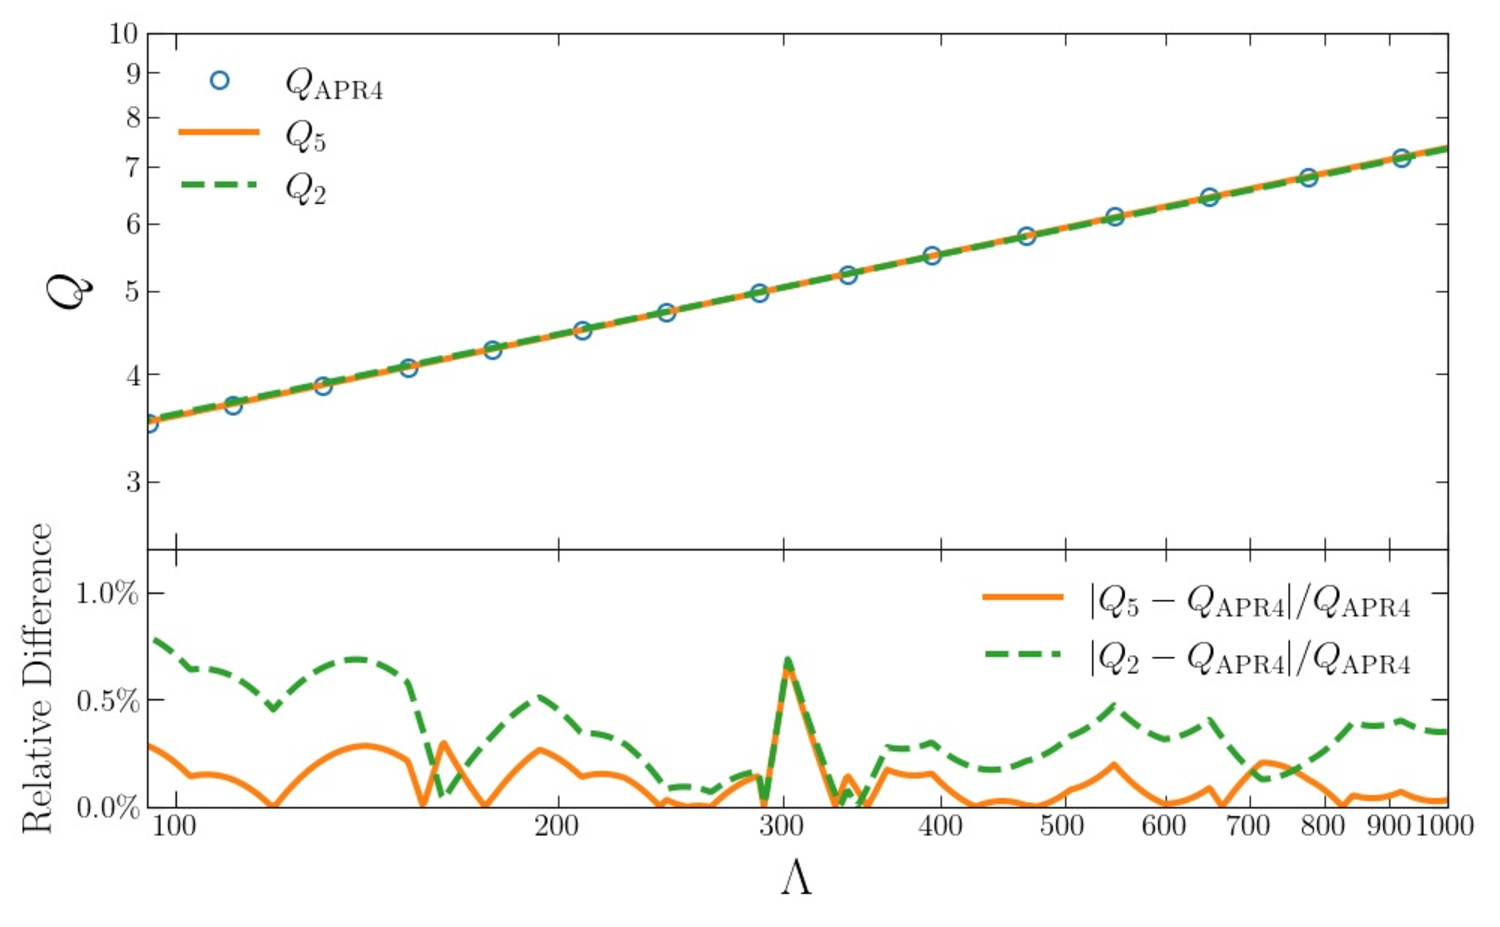
\includegraphics[width=0.8\textwidth]{2d-5d difference.pdf}% Here is how to import EPS art
\caption{Illustration of the Love-Q relation. In the upper panel, the orange
solid line indicates the original Yagi-Yunes relation, a quartic polynomial model
 in
Eq.~\eqref{5-d_Love_Q_eq}, while the green dashed line represents our fitting
with the linear model in Eq.~\eqref{2-d_Love_Q_eq}. We also show the Love-Q
relation in the case of APR4 EOS for reference, plotted with blue circles.
In the lower panel, we show the absolute relative differences of the quadrupole
moments
between the two
models (denoted as $Q_5$ and $Q_2$) and the APR4 EOS (denoted as $Q_{\rm
APR4}$), respectively.}\label{relative_difference}
\end{figure}

%=============================
\subsection{Principles}
\label{subsec:framework_principles}
%=============================

The coefficients in Eq.~\eqref{5-d_Love_Q_eq} and Eq.~\eqref{2-d_Love_Q_eq} 
do not contribute directly to the GW waveform. Instead, they 
determine a relation between the waveform parameters
$\Lambda$ and $Q$, denoted as $Q=f(\Lambda;\bm{H})$, where $\bm{H}$ represents
the coefficients, $\bm{H} = \{a_2, b_2\}$ or $\bm{H} = \{a_5, b_5, c_5, d_5,
e_5\}$.
This leads to a delta-function-type prior between GW parameters $\Lambda$ and $Q$
\begin{equation}
\label{delta function prior}
\pi(Q|\Lambda,\bm{H}) = \delta\big(Q-f(\Lambda;\bm{H})\big)\,.
\end{equation}
Intuitively, one can measure $\Lambda$ and $Q$ from BNS GW events, and then fit
the relation with the measurements. This procedure can be implemented within the
hierarchical Bayesian framework, which is a powerful formalism in studying population
properties of GW events beyond individual observations~\cite{Thrane_2019}. The
population properties, 
are characterized by a set of hyperparameters, such as the power index of the
mass distribution. These hyperparameters do not enter the waveform directly,
while can only be inferred from a collection of measurements of single-event
parameters. Similarly, the EOS parameters determine the relation between the
$\Lambda-m$ relation and the $Q-m$ relation, and can be regarded as
hyperparameters and analyzed in the hierarchical Bayesian
framework~\cite{Mandel:2009nx,Mandel:2009pc,Adams:2012qw,Lackey:2014fwa,Mandel:2018mve,Golomb:2021tll,KAGRA:2021duu,Wang:2024xon}. In this work,
we adopt this framework to the inference of the Love-Q relation.


In this subsection, we briefly introduce the hierarchical Bayesian framework and
describe the customization in inferring the Love-Q relation.
The hierarchical Bayesian framework aims to
find the posterior distribution of the hyperparameters $p(\bm{H}|D)$, give the
catalog-level data $D=\{d_1,\cdots,d_n\}$ consisting of $n$ individual GW events.
Since both the hyperparameters $\bm{H}$ and the single-event parameters
$\{\bm{\theta}_1,\cdots,\bm{\theta}_n\}$ are unknown, we write the Bayes'
theorem as 
\begin{equation}
\label{bayes2}
p(\bm{H},\bm{\theta}_1,\cdots,\bm{\theta}_n|D)=\frac{p(D|\bm{H},\bm{\theta}_1,\cdots,\bm{\theta}_n)\pi(\bm{H},\bm{\theta}_1,\cdots,\bm{\theta}_n)}{p(D)}\,,
\end{equation}
where $\pi(\bm{H},\bm{\theta}_1,\cdots,\bm{\theta}_n)$ is the prior, $p(D|\bm{H},\bm{\theta}_1,\cdots,\bm{\theta}_n)$ 
is the likelihood function, and $p(D)$ denotes the evidence. Then, $p(\bm{H}|D)$
can be obtained by 
marginializing over the single-event parameters
\begin{equation}
\label{bayes1}
p(\bm{H}|D) = \int p(\bm{H},\bm{\theta}_1,\cdots,\bm{\theta}_n|D) \text{d}\bm{\theta}_1\cdots\text{d}\bm{\theta}_n\,,
\end{equation}

Assuming that the $n$ events are independent, the 
prior can be decomposed into parts of hyperparameters and single-event parameters,
\begin{equation}
\label{bayes3}
\pi(\bm{H},\bm{\theta}_1,\cdots,\bm{\theta}_n) = \pi(\bm{H}) \prod_{i=1}^n \pi(\bm{\theta}_i|\bm{H})\,.
\end{equation}
Since we are inferring the Love-Q relation, the tidal deformabilities $\bm
{\Lambda}_i=\{\Lambda_{1i},\Lambda_{2i}\}$ and quadrupole moments $\bm{Q}_i=\{Q_
{1i},Q_{2i}\}$ \ZW{I still recommend to use $Q^{(i)}_1$ and $Q^{(i)}_2$ for a
more clearer notation. But maybe current description does not cause confusion.
What's others' opinion?
} of the two NSs of the $i\text{-th}$ event are treated as independent
parameters in $\bm{\theta}_i$. Note that Love-Q relation is insensitive 
to the EOS, the prior of mass parameters $m_1$ and $m_2$ are chosen to be
independent of $\bm{\Lambda}_i, \bm{Q}_i$ and $\bm{H}$. Other parameters in
$\bm{\theta}_i$ are also assumed to be independent chosen. 
In this way, the conditional prior of $\bm{\theta}_i$
 can be further decomposed as
\begin{equation}
\label{prior}
\pi(\bm{\theta}_i|\bm{H})=\pi(\bm{\Lambda}_i|\bm{H})\pi(\bm{Q}_i|\bm{\Lambda}_i,\bm{H})\times\pi(\bm{\xi}_i)\,,
\end{equation}
where $\bm{\xi}_i$ denotes the other parameters in $\bm{\theta}_i$ except for
$\bm{\Lambda}_i$ and $\bm{Q}_i$, called nuisance parameters hereafter.
Analogously to the prior, the catalog likelihood can be factorized
 into the product of single-event likelihoods
\begin{equation}
    p(D|\bm{H},\bm{\theta}_1,\cdots,\bm{\theta}_n)=\prod_{i=1}^{n}p(d_i|\bm{H},\bm{\theta}_i)=\prod_{i=1}^{n}p(d_i|\bm{\theta}_i)\,,\label{eq:catalog_likelihood}
\end{equation}
where the second equality comes from the fact that the hyperparameters do not enter the waveform.

Given the specific form of the prior and the likelihood, the marginalized posterior distribution (Eq.~\eqref{bayes1}) becomes
\begin{equation}
\label{hierarchical bayes}
\begin{aligned}
p(\bm{H}|D)&=\frac{1}{p(D)}\pi(\bm{H})\int \text{d}\bm{\theta}_1\cdots\text{d}\bm{\theta}_n \prod_{i=1}^n \big[\pi(\bm{\Lambda}_i|\bm{H})\pi(\bm{Q}_i|\bm{\Lambda}_i,\bm{H})\pi(\bm{\xi}_i)p(d_i|\bm{\theta}_i)\big] \\
&=\frac{1}{p(D)} \pi(\bm{H}) \prod_{i=1}^n
\int \text{d}\bm{\Lambda}_i\text{d}\bm{Q}_i\pi(\bm{\Lambda}_i|\bm{H})\delta\big(\bm{Q}_i-\bm{f}(\bm{\Lambda}_i;\bm{H})\big) \int \text{d}\bm{\xi}_i \pi(\bm{\xi}_i)p(d_i|\bm{\theta}_i)\\
&=\frac{1}{p(D)} \pi(\bm{H}) \prod_{i=1}^n
\int \text{d}\bm{\Lambda}_i\pi(\bm{\Lambda}_i|\bm{H})L_i\big(\bm{\Lambda}_i,\bm{f}(\bm{\Lambda}_i;\bm{H})\big)\,.
\end{aligned}
\end{equation}
In the second line, the bold font $\bm{f}(\bm{\Lambda}_i;\bm{H})$ is used to denote the vector form
of the Love-Q relation applied to the two NSs in a BNS system. In the third line,
$L_i(\bm{\Lambda}_i,\bm{Q}_i)$, called the quasi-likelihood,
 is defined as the integral over the nuisance
parameters
\begin{equation}
\label{quasi-likelihood}
    L_i(\bm{\Lambda}_i,\bm{Q}_i)=\int \text{d}\bm{\xi}_i \pi(\bm{\xi}_i)p(d_i|\bm{\theta}_i)\,.
\end{equation}

The quasi-likelihood of each event can be 
computed independently of $\bm{H}$. For the $i\text{-th}$ event, we write down
the Bayes' theorem
\begin{equation}
\label{single bayes}
    p(\bm{\theta}_i|d_i, \varnothing)\propto \pi(\bm{\theta}_i|\varnothing)p(d_i|\bm{\theta}_i)\,,
\end{equation}
where $\pi(\bm{\theta}_i|\varnothing)$ denotes an auxiliary prior 
independent of $\bm{H}$. $p(d_i|\bm{\theta}_i)$ is the single-event
likelihood (same as in Eq.~\eqref{eq:catalog_likelihood}), whose explicit form is
 given by assuming stationary, Gaussian noise~\cite{Finn:1992wt}
\begin{equation}
p(d_i|\bm{\theta}_i)\propto \mathrm{e}^{-\frac{1}{2}\langle d_i-h(\bm{\theta}_i),d_i-h(\bm{\theta}_i)\rangle}\,,
\end{equation}
with the data $d_i$ and the waveform model $h(\bm{\theta}_i)$. $\langle u, v\rangle$ 
is the inner product of $u(t)$ and $v(t)$ weighted by the power spectrum density
(PSD) of $S_n(f)$ of the noise, defined as
\begin{equation}
    \langle u, v\rangle:= 2\int_{-\infty}^{\infty}\frac{\tilde{u}(f)\tilde{v}^{*}(f)}{S_n(|f|)} \text{d}f\,,
\end{equation}
where $\tilde{u}(f)$ and $\tilde{v}(f)$ are the Fourier transforms of $u(t)$ and $v(t)$.

Rearranging terms of Eq.~\eqref{single bayes} and substituting it into
Eq.~\eqref{quasi-likelihood}, one finds that
\begin{equation}
\label{quasi-posterior}
\begin{aligned}
    L_i(\bm{\Lambda}_i,\bm{Q}_i) = \int \text{d}\bm{\xi}_i \pi(\bm{\xi}_i)p(d_i|\bm{\theta}_i) \propto \int \text{d}\bm{\xi}_i \frac{\pi(\bm{\xi}_i)}{\pi(\bm{\theta}_i|\varnothing)}p(\bm{\theta}_i|d_i,\varnothing)\,.
\end{aligned}  
\end{equation}
If we further choose $\pi(\bm{\theta}_i|\varnothing)\propto\pi(\bm{\xi}_i)$, 
i.e., a flat prior for $\bm{\Lambda}_i$ and $\bm{Q}_i$, Eq.~\eqref{quasi-posterior} can be further simplified as 
\begin{equation}
\label{quasi-marginalized}
\begin{aligned}
    L_i(\bm{\Lambda}_i,\bm{Q}_i) \propto \int \text{d}\bm{\xi}_i p(\bm{\theta}_i|d_i,\varnothing)\propto p(\bm{\Lambda}_i,\bm{Q}_i|d_i,\varnothing)\,.
\end{aligned}  
\end{equation}
This means that the quasi-likelihood is proportional to the marginalized
posterior of the auxiliary single-event inference with a flat prior on
$\bm{\Lambda}_i$ and $\bm{Q}_i$. The
hierarchical Bayesian framework, as its name implies, introduces two levels of 
inferences. The first level 
consists of single-event Bayesian inferences based on Eq.~\eqref{single bayes},
where the quasi-likelihoods are constructed according to
Eq.~\eqref{quasi-marginalized}. In the second level, the quasi-likelihoods are
combined to infer the hyperparameters based on Eq.~\eqref{hierarchical bayes}.


%=============================
\section{Simulation}
\label{sec:simulation}
%=============================

%=============================
\subsection{Waveform, Population and Detectors}
\label{subsec:simulation_preliminaries}
%=============================

In our simulation, we adopt the {\sc IMRPhenomXAS\_NRTidalv3} waveform model~\cite{Abac:2023ujg}, 
which includes tidal amplitude corrections as well as spin-induced quadrupole
moment terms up to 3.5PN with aligned spins.
The single-event parameters $\bm{\theta}$ include 
 the binary masses $m_1$ and $m_2$, the 
dimensionless tidal deformabilities $\Lambda_1$ and $\Lambda_2$, spin-induced 
quadrupole moments $Q_1$ and $Q_2$, the dimensionless spin $\chi_1$ and $\chi_2$, the 
luminosity distance $D_L$, the merge time $t_c$, the right ascension $\alpha$ and 
declination $\delta$, the inclination angle $\iota$, the GW polarization angle 
$\psi$ and the phase of coalescence $\phi_c$.

When generating the BNS events, we adopt the population model proposed by \citet{Farrow:2019xnc}. 
According to their spin magnitude, the model divides BNS into a recycled star and a nonrecycled 
(\emph{slow}) one, for which the masses are labeled $m_r$ and $m_s$, respectively. 
The distribution of $m_r$ has two Gaussian components while $m_s$ follow a uniform distribution,
\begin{subequations}
\label{mass population}
\begin{equation}
    P(m_{\mathrm{r}}) = \alpha \mathcal{N}(\mu_1, \sigma_1) + (1-\alpha) \mathcal{N}(\mu_2, \sigma_2)\,,
\end{equation}
\begin{equation}
    P(m_{\mathrm{s}}) = \mathcal{U}(m_{\mathrm{s}}^l, m_{\mathrm{s}}^u)\,,
\end{equation}
\end{subequations}
where $\alpha=0.68$, $\mu_1=1.34\,\mathrm{M}_{\odot}$, $\sigma_1=0.02\,\mathrm{M}_
{\odot}$, $\mu_2=1.47\,\mathrm{M}_{\odot}$, $\sigma_2=0.15\,\mathrm{M}_{\odot}$ 
and $m_{\mathrm{s}}^l=1.14\,\mathrm{M}_{\odot}$, $m_{\mathrm{s}}^u=1.46\,\mathrm{M}_{\odot}$. Then, the NS with a larger mass is labeled as the primary star with mass $m_1$ and the other as the secondary star with mass $m_2$.
The tidal deformability and quadrupole moments of the binary are calculated from 
the stellar mass assuming the APR4 EOS with methods described in Refs.~\cite{Yagi:2013awa,Atta:2024ckt}. For the spin of recycled stars $\chi_r$, we adopt a uniform distribution $\mathcal{U}(-0.5,0.5)$, 
while for $\chi_s$ we draw from $\mathcal{U}(-0.1,0.1)$.
Using the cosmological parameters provided by the Planck Collaboration~\cite{Planck:2018vyg}, 
we simulate 1000 gravitational wave (GW) sources, a total number estimated from the observed local merger rate 
$7.6$--$250\,\mathrm{Gpc}^{-3}\mathrm{yr}^{-1}$ from current GW detections~\cite{LIGOScientific:2025pvj,LIGOScientific:2020aai}. 
These sources are distributed uniformly in source-frame time and co-moving volume between 15~Mpc and 150~Mpc, 
with isotropic sky locations and orientations. Without loss of generality, all GW events are injected with $t_c=0$.

We select a XG detector network consisting of two CE detectors and one ET 
detector, whose sensitivities are taken as CE-2~\cite{Reitze:2019iox,Reitze:2019dyk} 
and ET-D~\cite{Punturo:2010zz,Hild:2010id,Sathyaprakash:2012jk}, respectively. 
The two CE detectors are positioned at the current sites of the two LIGO detectors, 
while the ET detector is set at the current location of the Virgo detector with a triangular shape. 

%=============================
\subsection{Implementation}
\label{subsec:simulation_implementation}
%=============================

According to the discussion in section~\ref{subsec:framework_principles}, the inference of the Love-Q relation
can be divided into two steps.
In the auxiliary single-event inference, the variable parameters are $\bm{\theta} = \{\mathcal{M},\eta,
\Lambda_1,\Lambda_2,Q_1,Q_2,\chi_1,\chi_2,D_L,t_c,\alpha,\delta,\iota,\psi,\phi_c\}
$. The priors of $\mathcal{M}$, $\eta$, $\chi_1$, $\chi_2$, $t_c$ and $\phi_c$ are uniform, and
the prior of $D_L$ is uniform in source frame time and co-moving volume. We 
set isotropic priors for the angle variables $\alpha,\delta,\iota,\psi$. For tidal 
and quadrupole moment parameters, we treat $\Lambda_s$ and $Q_s$ of the slow 
binary component as nuisance parameters, since the spin-induced 
quadrupole moment is poorly estimated for NSs with low spins~\cite{Yagi:2013awa}.
According to the arguments around Eq.~\eqref{quasi-marginalized}, we choose
uniform priors for $\Lambda_1$, $\Lambda_2$, $Q_1$ and $Q_2$ in the auxiliary inference.
For calculating the posterior, we generate samples with the {\sc
Bilby}~\cite{Ashton:2018jfp} implementation of the {\sc nessai}
sampler~\cite{Skilling:2004pqw,Skilling:2006gxv,michael_j_williams_2025_14627250,PhysRevD.103.103006,Williams:2023ppp}.
To calculate the integral in Eq.~\eqref{hierarchical bayes}, we need the
fuctional form of the quasi-likelihood, which is proportional to the
distribution function of the posterior
$p(\bm{\Lambda}_i,\bm{Q}_i|d_i,\varnothing)$. We follow
\citet{Golomb:2021tll} and adopt the Gaussian mixture 
model to estimate the density of the posterior samples.
In the second step, the priors of the hyperparameters $\pi(\bm{H})$ are listed
in table~\ref{prior_table}. For the conditional prior $\pi(\bm
{\Lambda}_i|\bm{H})$, we choose the uniform distribution $\mathcal{U}(10,2000)$. 

We simulate 1000 GW events as 
described in section~\ref{subsec:simulation_preliminaries}. 
Though the hierarchical procedure avoids a direct high-dimensional inference for
$\bm{H}$ and $\{\bm{\theta}_1,\cdots,\bm{\theta}_n\}$ simultaneously, the
computational cost still increases with the number of events $n$.
\citet{Lackey:2014fwa} found that when constraining the EOS of NSs, several events
with the highest signal-to-noise ratios (SNRs)
 contribute most of the information. Also,
\citet{Yagi:2013awa} concluded that the spin-induced quadrupole moment can not
be well measured for NSs with low spins. Considering these findings, we first
draw 100 sources with the highest SNRs, then further select 20 sources with the
largest $|\chi_{r}|$ among them. As we will show in section~\ref{sec:results}, the primary
information for constraining the Love-Q relation comes from the 10 loudest GW
events. We leave a more comprehensive study of the whole population for future
work. 
\begin{table}[t]
    \centering
    \sisetup{
        table-align-text-post = false, 
        separate-uncertainty = true 
    }
        \caption{The reference values and priors of the coefficients in different models
        of the Love-Q relation, with $j$ being the number of parameters in
        the polynomial
        model. $j=5$ indicates the original Yagi-Yunes
        relation~\cite{Yagi_2017}. For $j = $ 2, 3 and 4, the values are
        the results of least squares regression performed on 1000 points uniformly sampled in logarithmic space from Yagi-Yunes relation. Priors are chosen to be uniform distributions, and the ranges
        are same for different $j$ to ensure a fair comparison.
        }\label{prior_table}
    \begin{tabular}{
        l
        S[table-format=-1.4]
        S[table-format=1.5]
        S[table-format=1.3e-1]
        S[table-format=-1.3e-1]
        S[table-format=1.3e-1]
    }
        \toprule
        \multicolumn{6}{c}{Reference values} \\
        %\cmidrule(l){2-6}
        $j$ & {$a_j$} & {$b_j$} & {$c_j$} & {$d_j$} & {$e_j$} \\
        \midrule

        5 \, &  0.1940 & 0.0916 & 4.812e-2 & -4.283e-3 & 1.245e-4 \\
        4 \, &  0.1290 & 0.1480  & 3.021e-2 & -1.817e-3 & {/}      \\
        3 \, & -0.0709 & 0.2775  & 3.220e-3 & {/}       & {/}      \\
        2 \, & -0.1457 & 0.3094  & {/}      & {/}       & {/}      \\
        
        \midrule

        \multicolumn{6}{c}{Priors} \\
        %\cmidrule(l){2-6}
        $j$ & {$a_j$} & {$b_j$} & {$c_j$} & {$d_j$} & {$e_j$} \\
        \midrule

        5 \, & {$\mathcal{U}(-5.0, 5.0)$} & {$\mathcal{U}(-1.0, 1.0)$} & {$\mathcal{U}(-0.5, 0.5)$} & {$\mathcal{U}(-0.1, 0.1)$} & {$\mathcal{U}(-0.01, 0.01)$} \\
        4 \, & {$\mathcal{U}(-5.0, 5.0)$} & {$\mathcal{U}(-1.0, 1.0)$} & {$\mathcal{U}(-0.5, 0.5)$} & {$\mathcal{U}(-0.1, 0.1)$} & {/}                         \\
        3 \, & {$\mathcal{U}(-5.0, 5.0)$} & {$\mathcal{U}(-1.0, 1.0)$} & {$\mathcal{U}(-0.5, 0.5)$} & {/}                       & {/}                         \\
        2 \, & {$\mathcal{U}(-5.0, 5.0)$} & {$\mathcal{U}(-1.0, 1.0)$} & {/}                       & {/}                       & {/}                         \\
        \bottomrule
    \end{tabular}
\end{table}


%=============================
\section{Results and Discussions}
\label{sec:results}
%=============================
%\ZW{I'm not recommend to use ``sec4'' to label the section, because it is not informative. Also for equation labels, since the index may change when you revise the paper, it is better to use some informative labels, e.g., ``sec:results and discussions''}
In this section, we present the inference results for different parameterization 
models of the Love-Q relation. In section~\ref{subsec:results_linear_model}, we 
show the results of the linear model, Eq.~\eqref{2-d_Love_Q_eq}, consisting of two parameters.
%\ZW{Another question: All eq. should be replaced by Eq. There is no additional ``.'' after figure and table, e.g., figure~\ref{corner2-d}, table~\ref{prior_table}.} 
In section~\ref{subsec:results_quartic}, we present the results of the quartic 
polynomial model in Eq.~\eqref{5-d_Love_Q_eq}, consisting of five parameters. The 
polynomial models in between, i.e., the quadratic and cubic polynomial models, are 
discussed in section~\ref{subsec:results_quadratic_cubic}.
%=============================
\subsection{Linear Model}
\label{subsec:results_linear_model}
%=============================
%\ZW{I delete ``fitting'', since it is not informative.}
\begin{figure}[t]
    \centering
    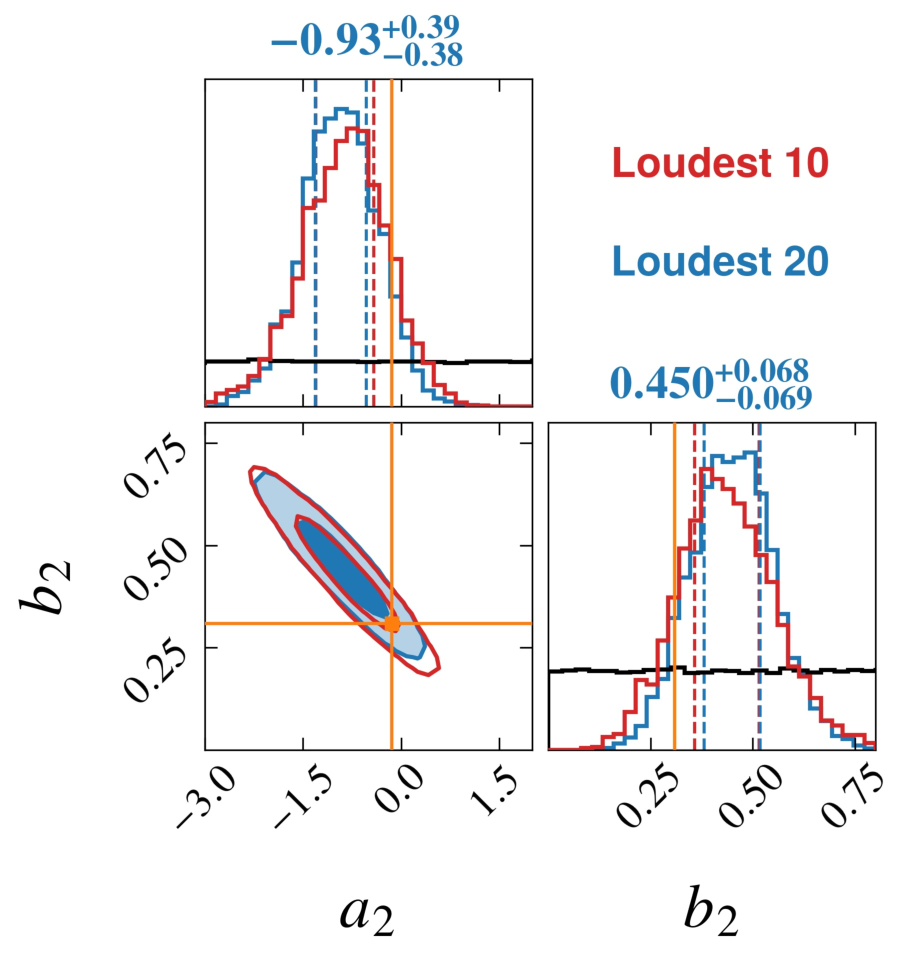
\includegraphics[width=0.5\linewidth]{comparison_corner_plot.pdf}
    \caption{Posterior of the hyperparameters ${\bm H} = \{a_2,b_2\}$
     in the linear fitting model. The contours refer to 50\% and 90\% credible
     regions, while the numbers above the histograms on the diagonal stand 
    for the median and the central 50\% credible interval of the marginalized
     distribution. We use blue and red colors to represent the results based on
     the loudest 20 and 10 events among the 1000
    simulated events, respectively.
     The orange lines represent the reference values in table~\ref{prior_table}.
     The black lines on the diagonal represent the priors for comparison.}
    \label{corner2-d}
\end{figure}


We first perform the inference for the linear model, which is also the model 
adopted in Ref.~\cite{Samajdar:2020xrd}. The posterior distribution of the 
hyperparameters $\{a_2,b_2\}$ is shown in figure~\ref{corner2-d}. Compared
to the priors in table~\ref{prior_table}, the posteriors are significantly 
narrowed. As a comparison, we also mark the fitting values of the hyperparameters 
in a direct fit of the Yagi-Yunes Love-Q relation, and regard them as ``true'' 
values of the linear model for reference. These values fall within the 90\% 
credible region of the posterior, and close to the marginal of the 50\% credible 
region. The hierarchical Bayesian inference successfully recovers the Love-Q 
relation under the linear parameterization. We also investigate how the results 
depend on the number of events in the analysis. In the 20 event selected in 
section~\ref{subsec:simulation_implementation}, we further select the loudest 10 
events, perform the inference again, and show the results in figure~\ref
{corner2-d}. For both the joint and marginalized distributions, the widths of the 
credible regions in the 10-event inference are only slightly larger than those in 
the 20-event inference. This reveals that the loudest 10 events dominate the 
information in constraining the Love-Q relation, and including quieter events will 
not significantly improve the results.


\begin{figure}[t]
\centering
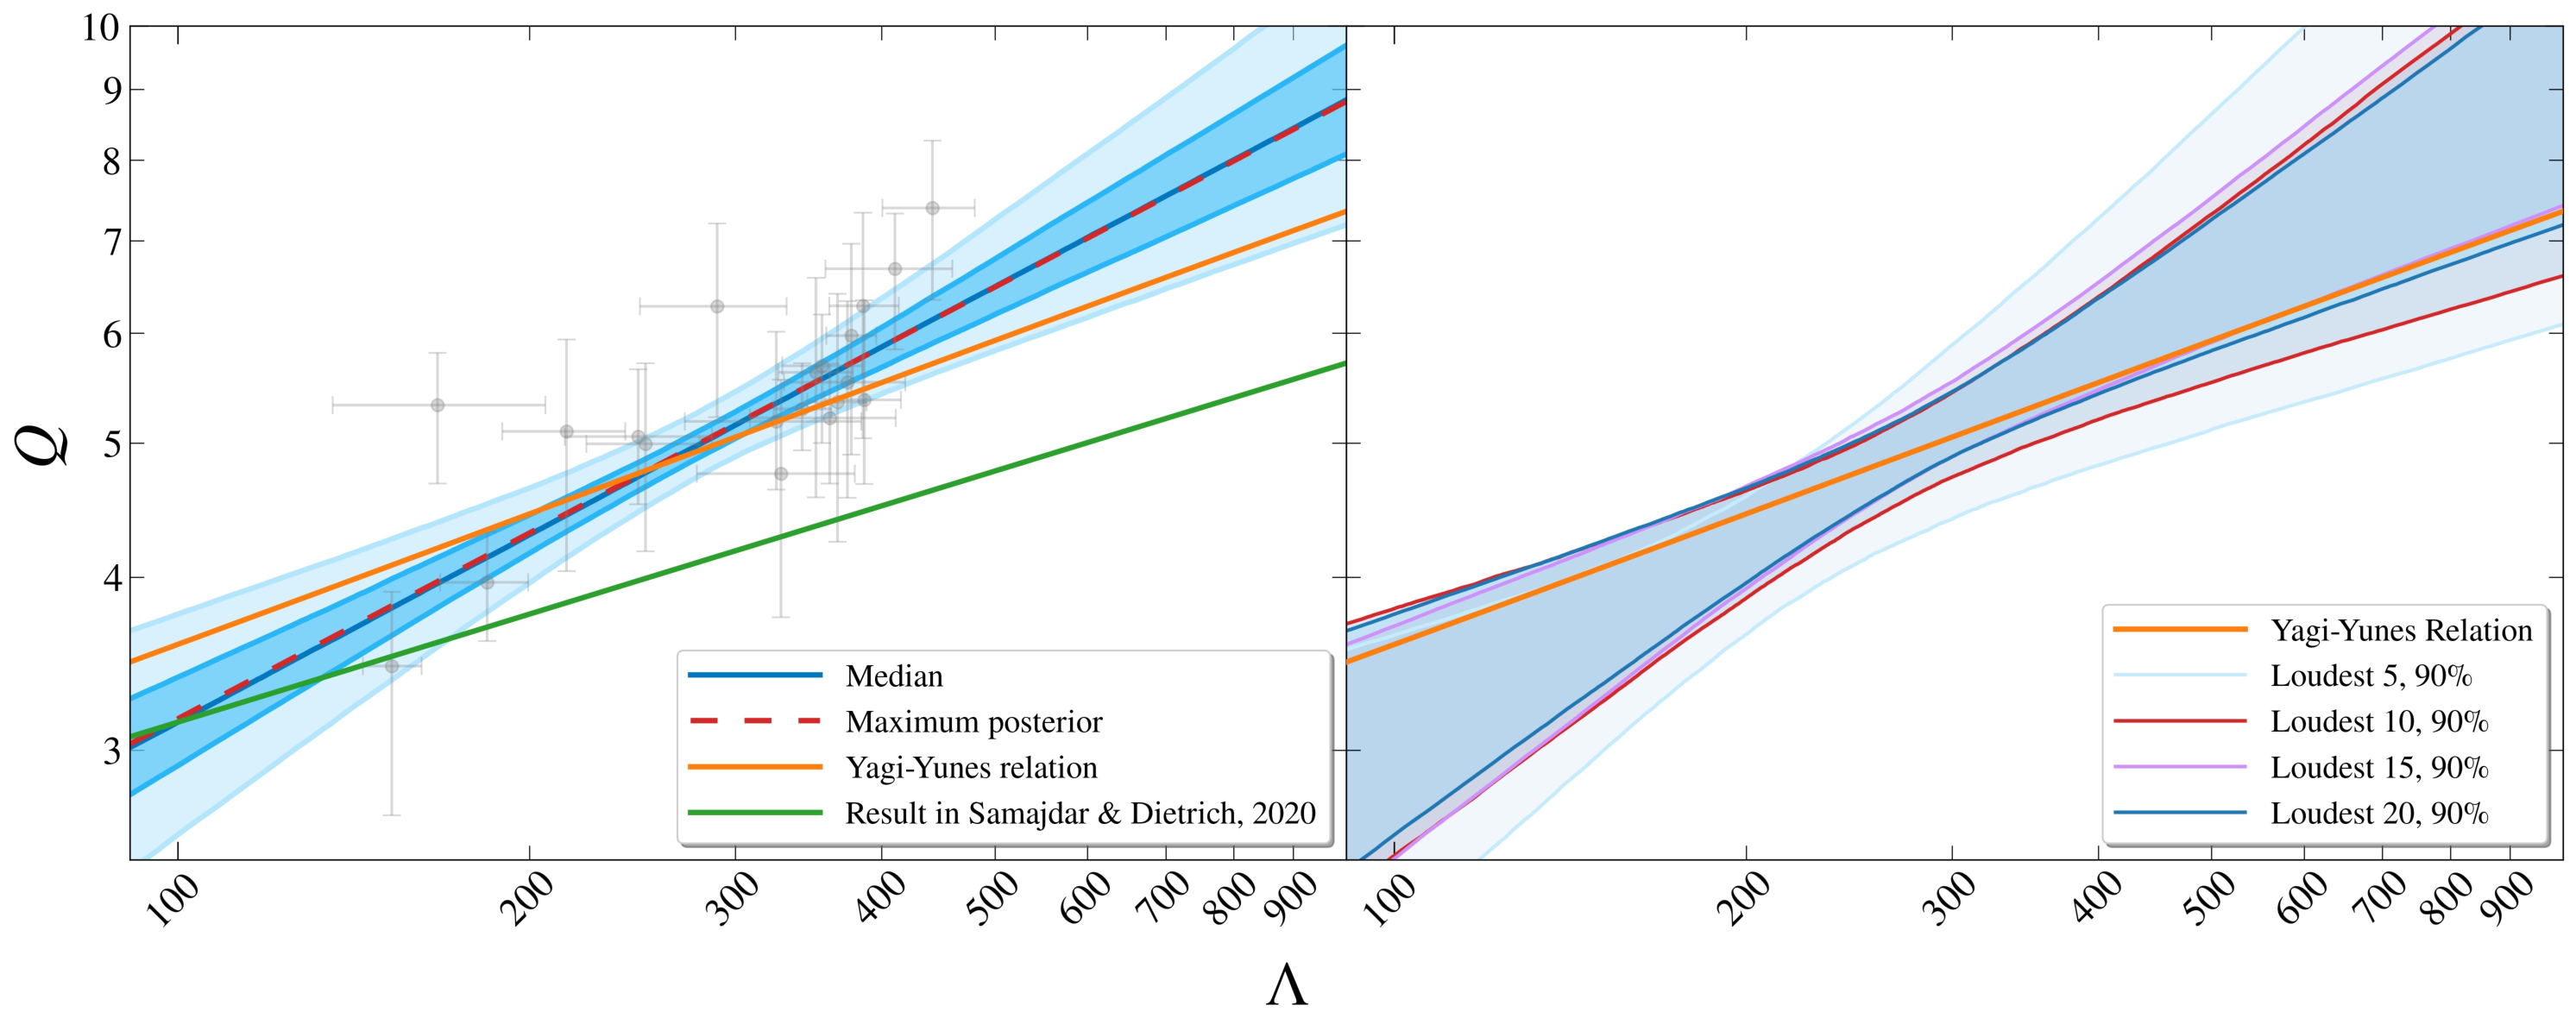
\includegraphics[width=\textwidth]{hierarchical_results_APR4_2d.pdf}
    \caption{Recovered Love-Q relation from the posterior of the hyperparameters
    in the linear model. In the left panel, the Love-Q relation is inferred with
    the 20 loudest events among the 1000
    simulated GW events. The gray points mark the median values of inferred
    $\Lambda$ and $Q$ for each event with $68\%$ error bars. The blue solid line
    marks the median of the distribution of $Q$ with certain $\Lambda$, accompanied
    by the $50\%$ and $90\%$ credible intervals represented in shaded regions.
    The red dashed line represents the maximum-posterior relation. For
    comparison, we plot the original Yagi-Yunes
    Love-Q relation~\cite{Yagi_2017} in orange and the recovered relation with
    linear regression in \citet{Samajdar:2020xrd}. The right panel shows how the
    $90\%$ credible region of the recovered Love-Q relation depends on the
    number of events, marked with different colors.}    \label{2-d_Love_Q}
\end{figure}

In figure~\ref{2-d_Love_Q}, we show the recovered Love-Q relation according to the 
posterior samples. For each $\Lambda$, every sample in the posterior of the 
hyperparameters corresponds to a $Q$ value. With $\Lambda$ fixed, we find the 
credible intervals of $Q$, and then vary $\Lambda$ continuously to form credible 
regions. In the left panel, we show the results of the 20-event inference. Similar 
to figure~\ref{corner2-d}, the Yagi-Yunes Love-Q relation iscovered by the 90\% credible region. 
In the right panel, we select the loudest 5, 10, 15 and 20 events from the 20 events to test how the recovered Love-Q relation 
depends on the number of events. We find the widths of the 90\% credible regions 
are almost the same for the 10, 15 and 20 event inferences. This is consistent 
with the posteriors in figure~\ref{corner2-d}, and again indicates that the 
loudest 10 events are almost sufficient to constrain the Love-Q relation. Similar 
phenomena were also found in previous studies~\cite{Lackey:2014fwa,Landry:2020vaw,Pang:2020ilf,Finstad:2022oni,Bandopadhyay:2024zrr,Wang:2024xon}, 
where the recovered $\Lambda$-$m$ relation were also dominated by the several loudest events.

%=============================
\subsection{Quartic Polynomial Model}
\label{subsec:results_quartic}
%=============================

\begin{figure}
\begin{minipage}[t]{0.49\textwidth}
\centering
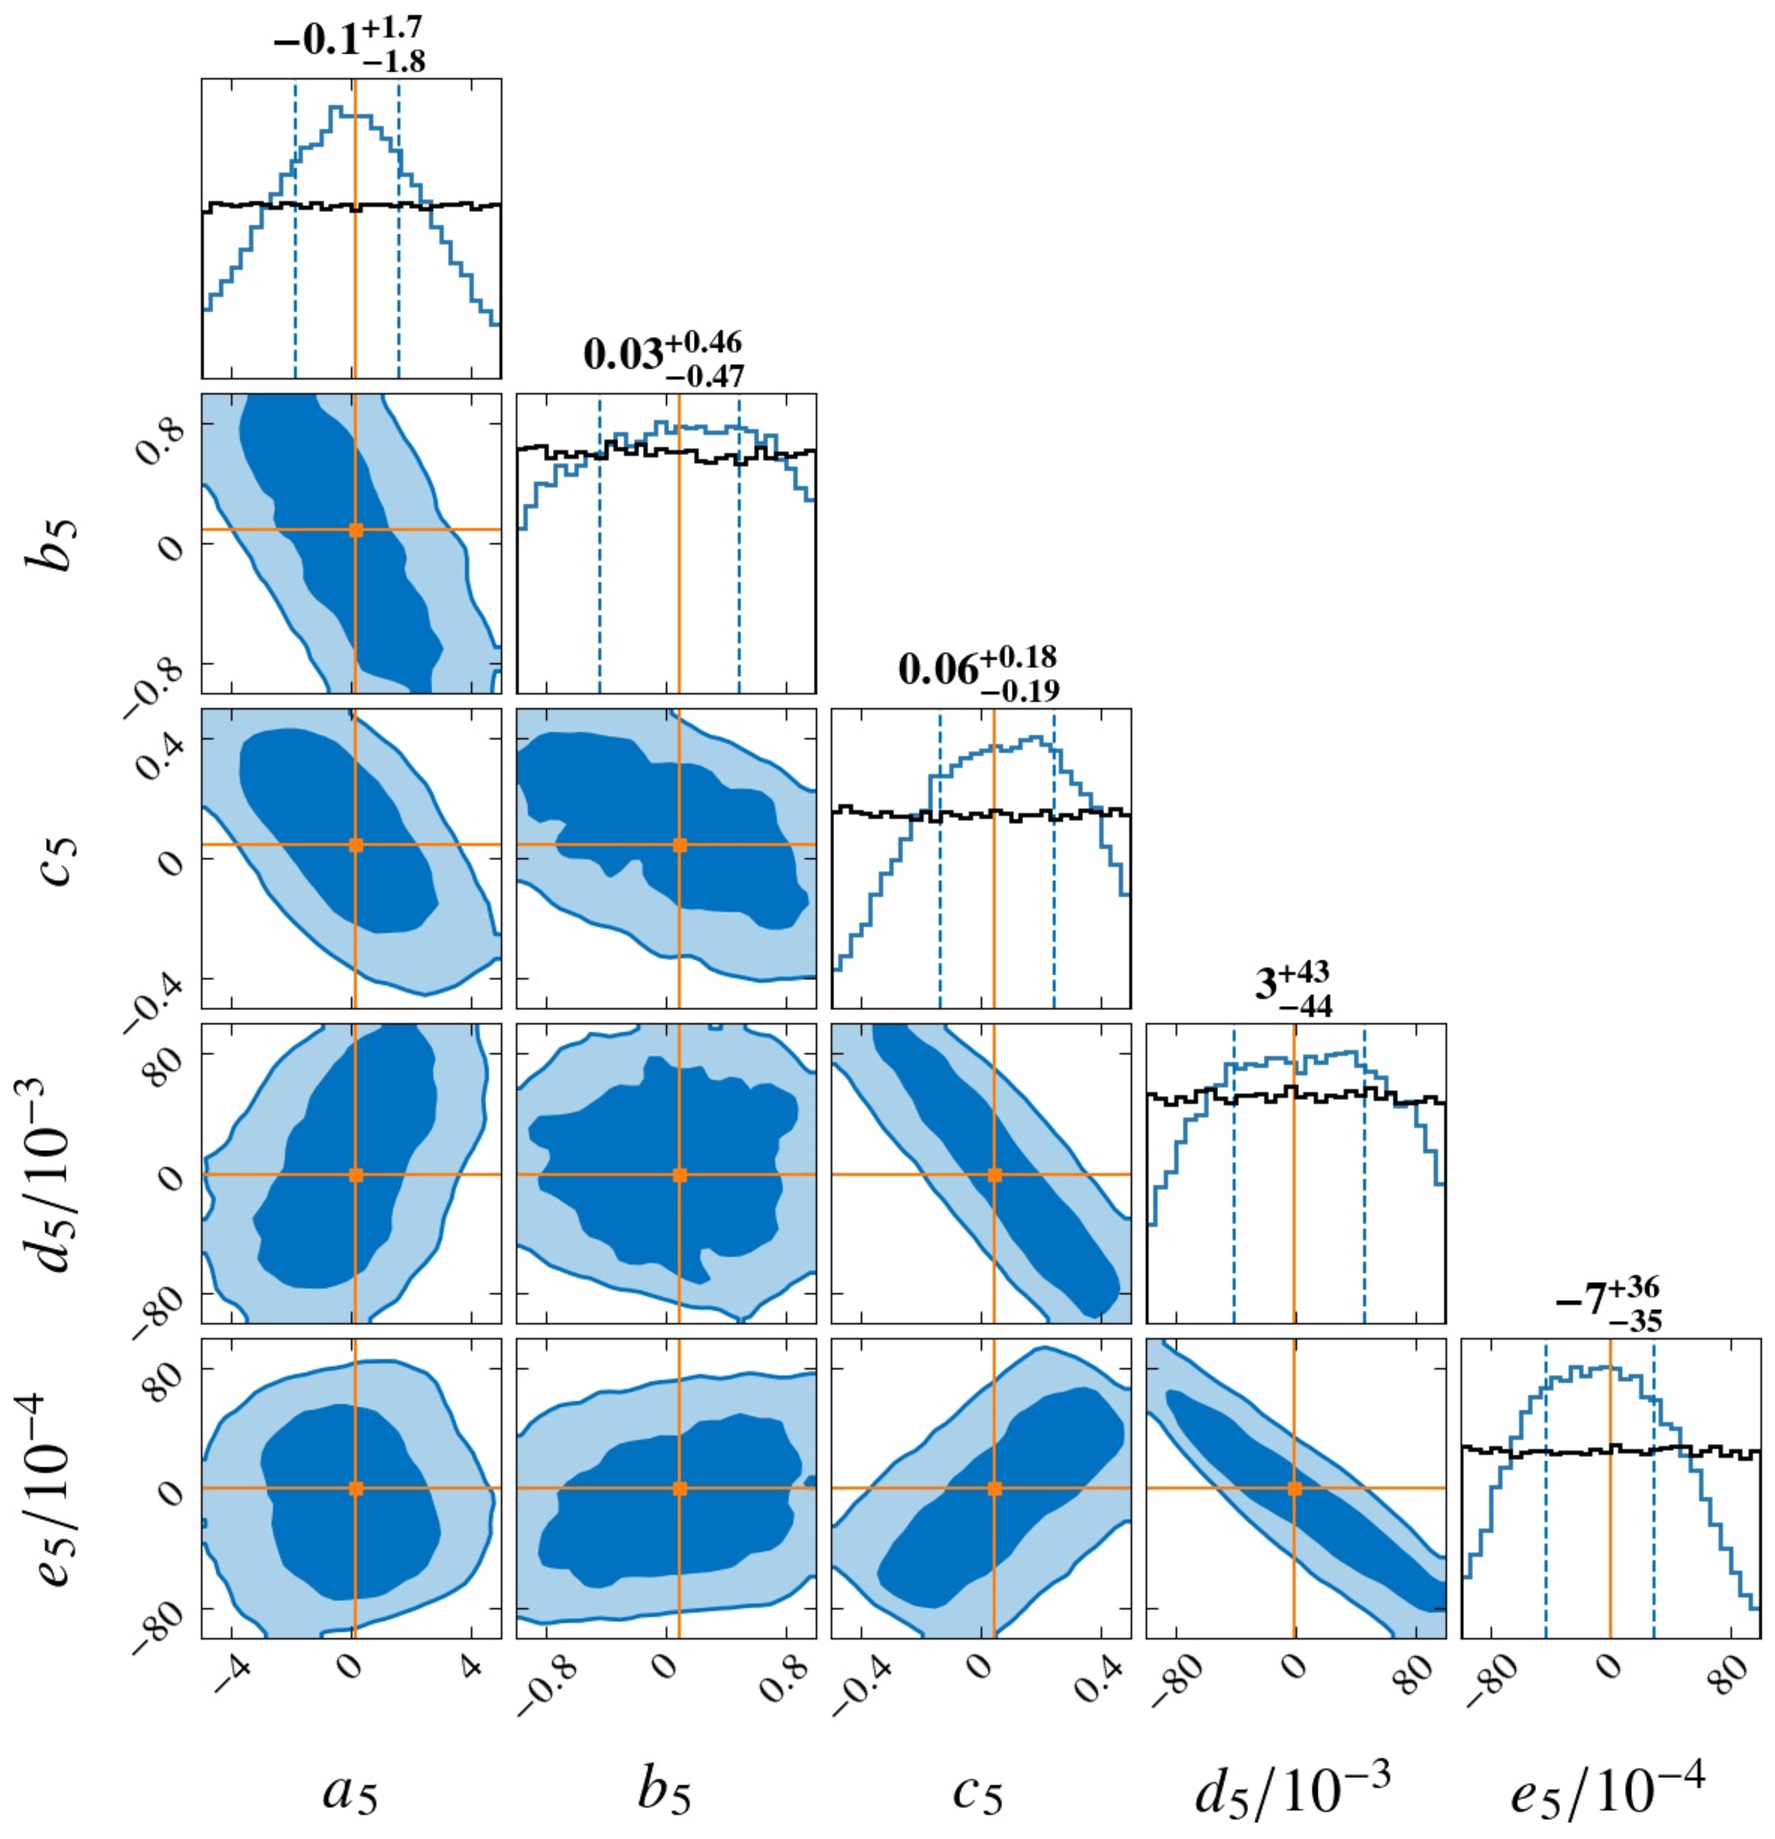
\includegraphics[width=0.8\linewidth]{Hyper_parameter_5d.pdf}% Here is how to import EPS art
\end{minipage}
\hfill
\begin{minipage}[t]{0.49\textwidth}
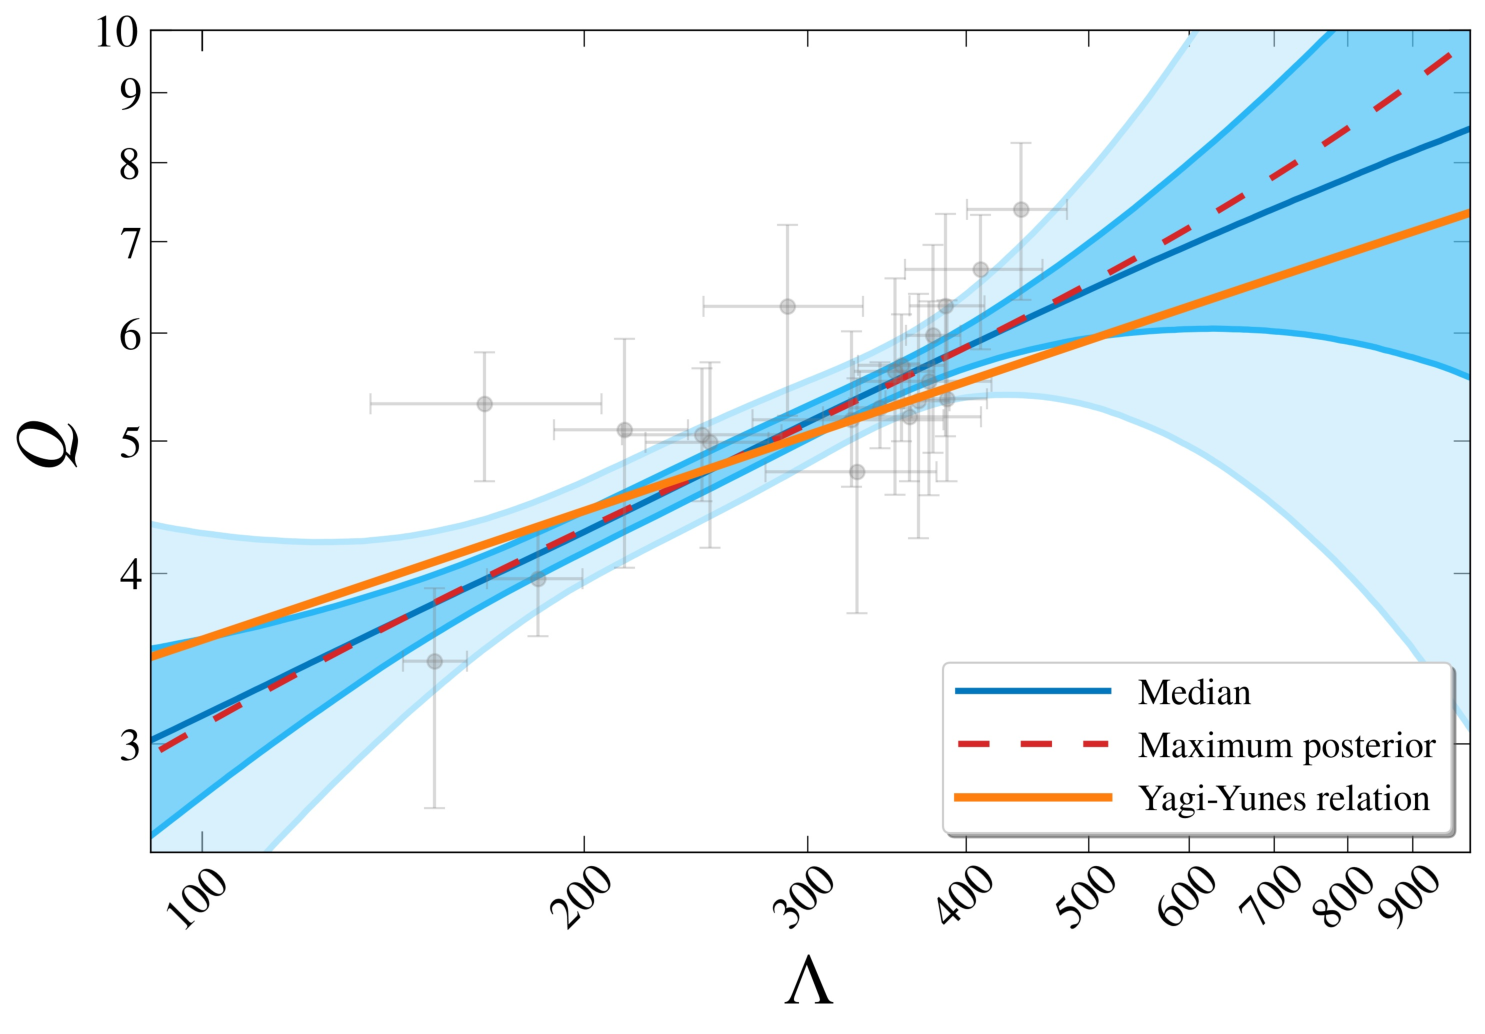
\includegraphics[width=\linewidth]{hierarchical_results_APR4_5d.pdf}
\end{minipage}
    \caption{The posterior of the hyperparameters and the recovered Love-Q relation
    in the quartic polynomial model, where all 20 loudest events are included in
    the inference. Plotting styles are similar to those in figure~\ref{corner2-d} and
    figure~\ref{2-d_Love_Q}.
    } \label{5-d_Love_Q} 
\end{figure}

For the quartic polynomial model, the Love-Q relation is fitted with five 
parameters shown in Eq.~\eqref{5-d_Love_Q_eq}, i.e., $\{a_5, b_5, c_5, d_5, e_5\}$. 
This is also the original model proposed by Yagi and Yunes~\cite{Yagi:2013awa}. We 
summarize the posterior and the recovered Love-Q relation in figure~\ref{5-d_Love_Q}, where
all 20 events are included in the inference. In the left panel, though the true 
values (the values in Yagi-Yunes Love-Q relation~\cite{Yagi:2013awa}) are almost 
centered in the 50\% and 90\% credible regions, the posteriors are much wider than 
those in the linear case, reaching the prior boundaries. This indicates that the $\Lambda$ and $Q$ measurements
from these events are not informative enough to well constrain all the five 
parameters. In other words, the observation precision is not high enough to 
capture the higher-order terms introduced by the additional three parameters
$c_5, d_5$ and $e_5$. This is also reflected in the strong correlations between 
the three parameter shown in the left panel of figure~\ref{5-d_Love_Q}. In the 
right panel of figure~\ref{5-d_Love_Q}, the 90\% credible regions of the
recovered Love-Q relation are also wider than those in the linear case, especially 
for large $\Lambda$ where the higher-order terms become more important. For 
$\Lambda \sim 400$, the widths of the 90\% credible region between
the two models are similar, which is consistent with the fact that most of the 
simulated events gather around this region. The Yagi-Yunes Love-Q relation is 
mostly covered by the 50\% credible region, and well within the 90\% credible region.

%=============================
\subsection{Quadratic and Cubic Polynomial Models}
\label{subsec:results_quadratic_cubic}
%=============================

\begin{figure}[t]
    \begin{minipage}[t]{0.49\textwidth}
    \centering
    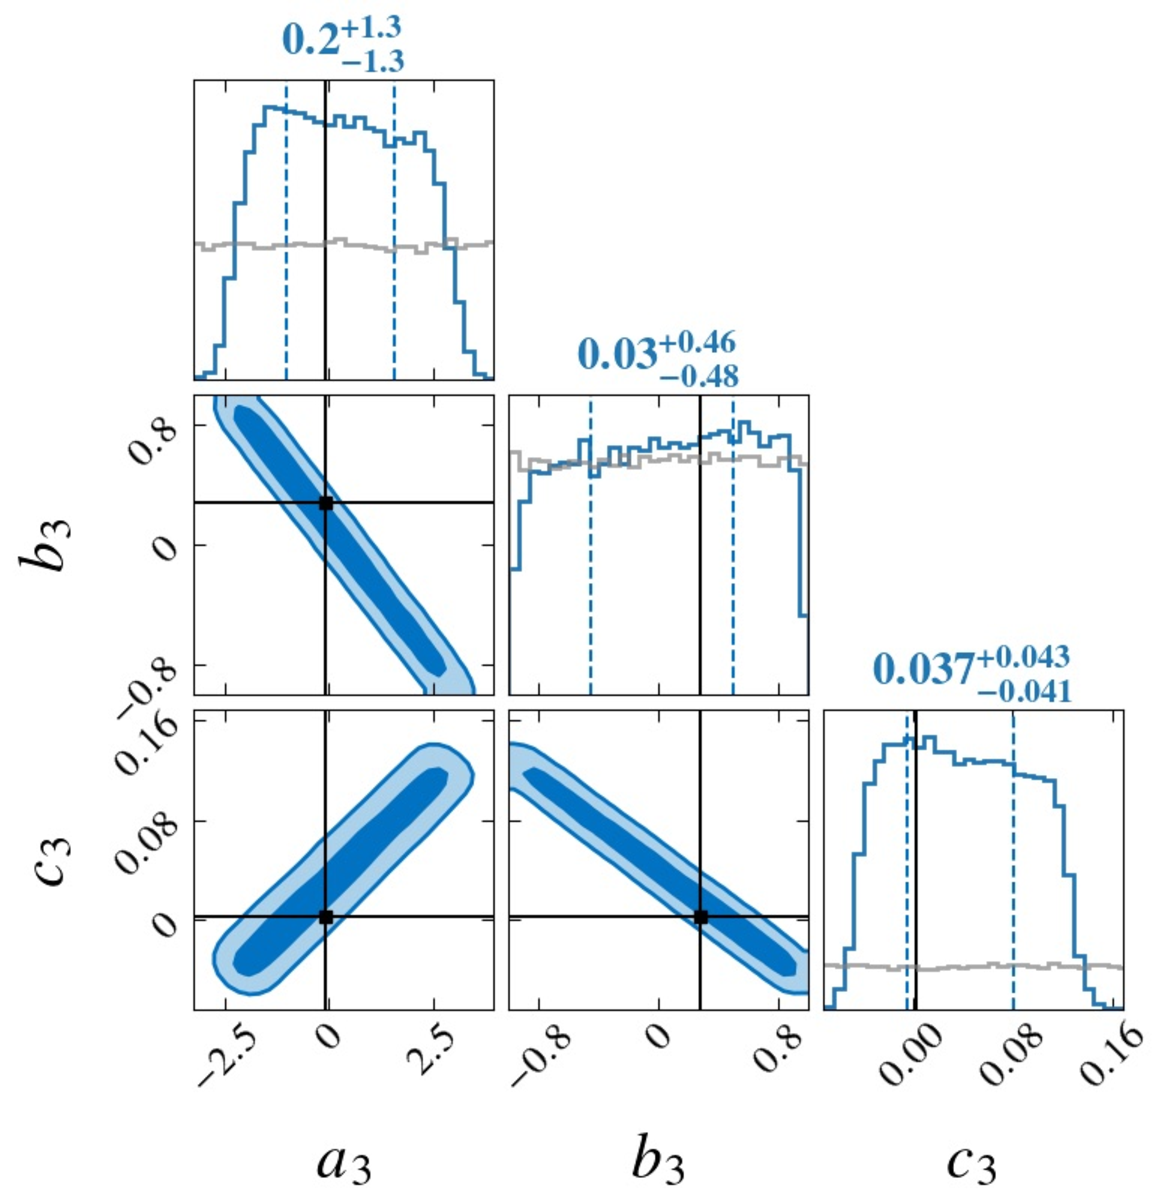
\includegraphics[width=0.8\linewidth]{Hyper_parameter_3d.pdf}
    \end{minipage}
    \hfill
    \begin{minipage}[t]{0.49\textwidth}
    \centering
    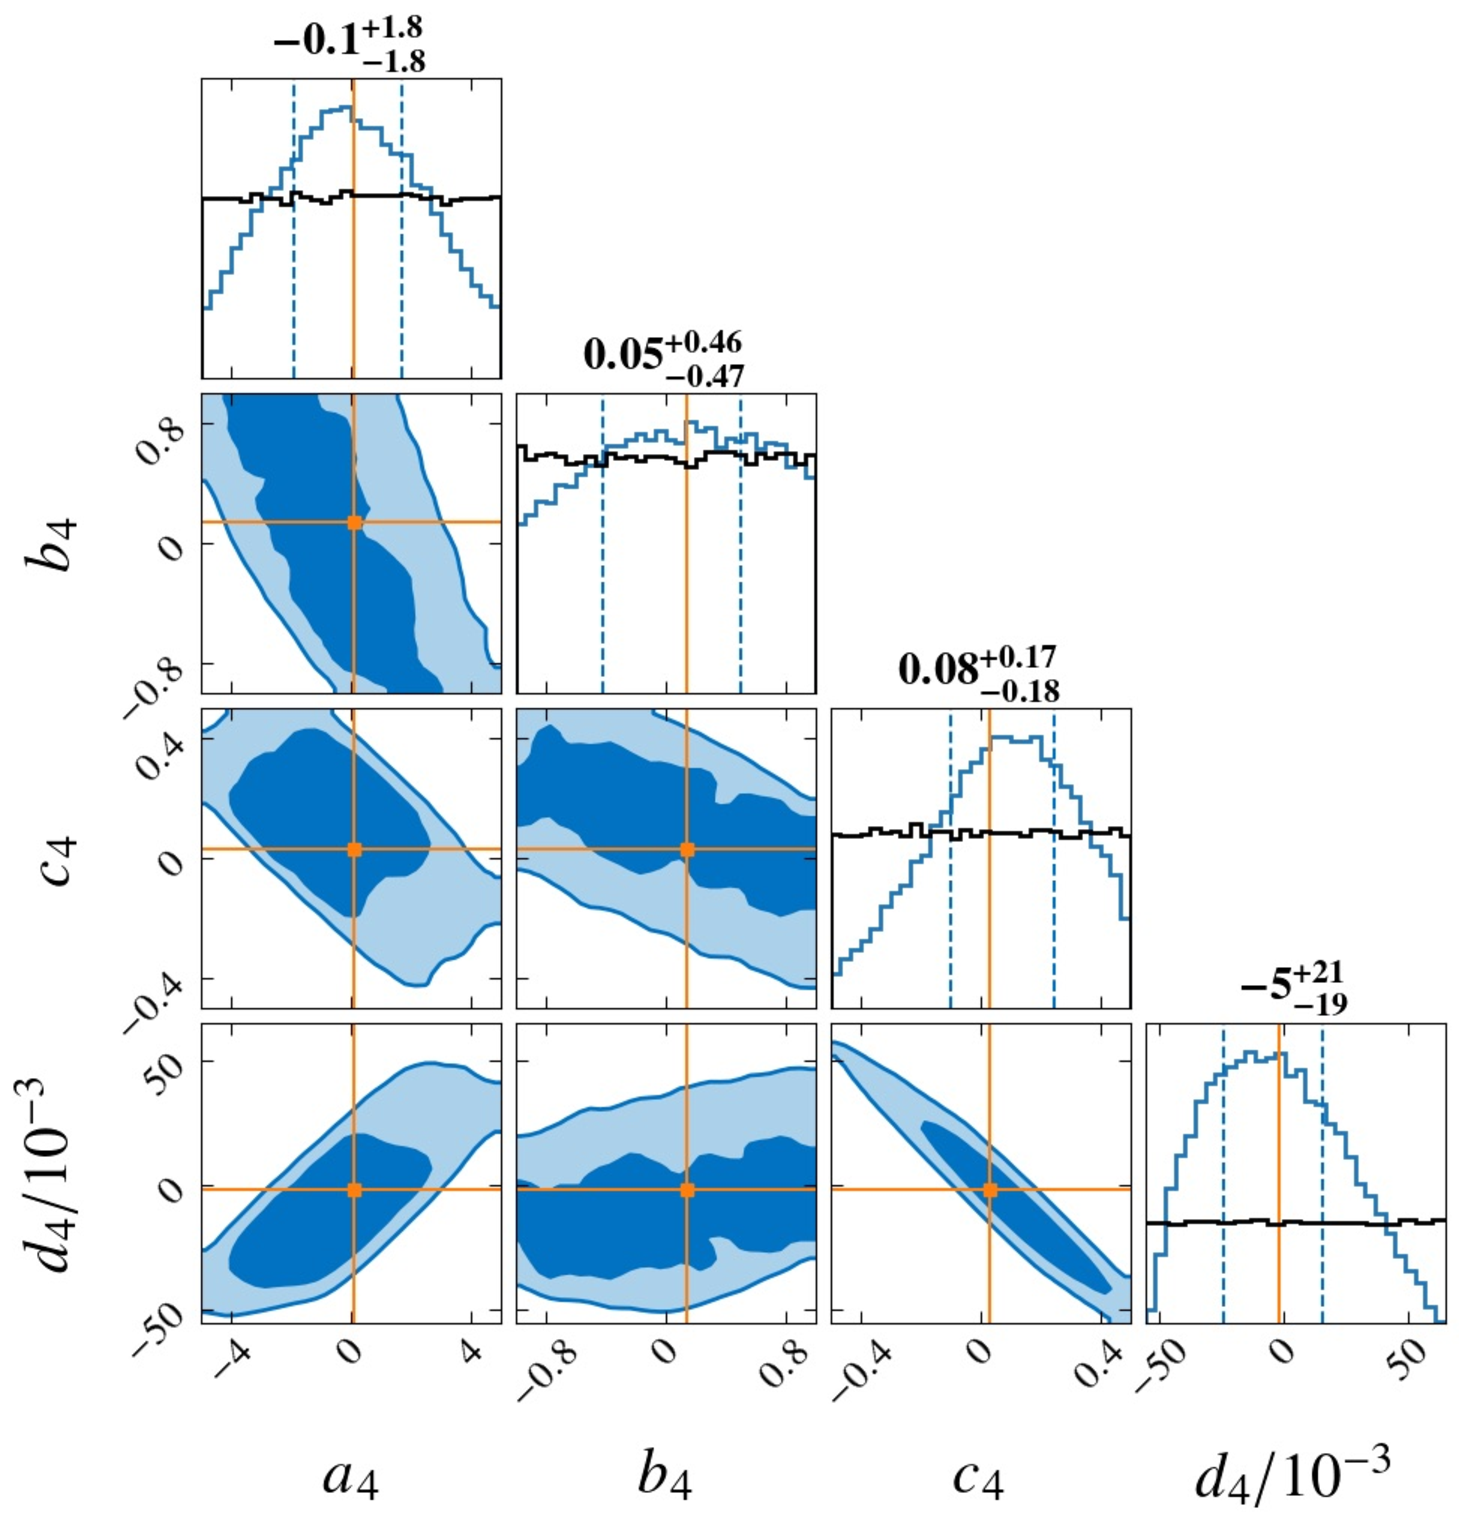
\includegraphics[width=0.8\linewidth]{Hyper_parameter_4d.pdf}
    \end{minipage}
    \vspace{3mm}
    \begin{minipage}[t]{\textwidth}
    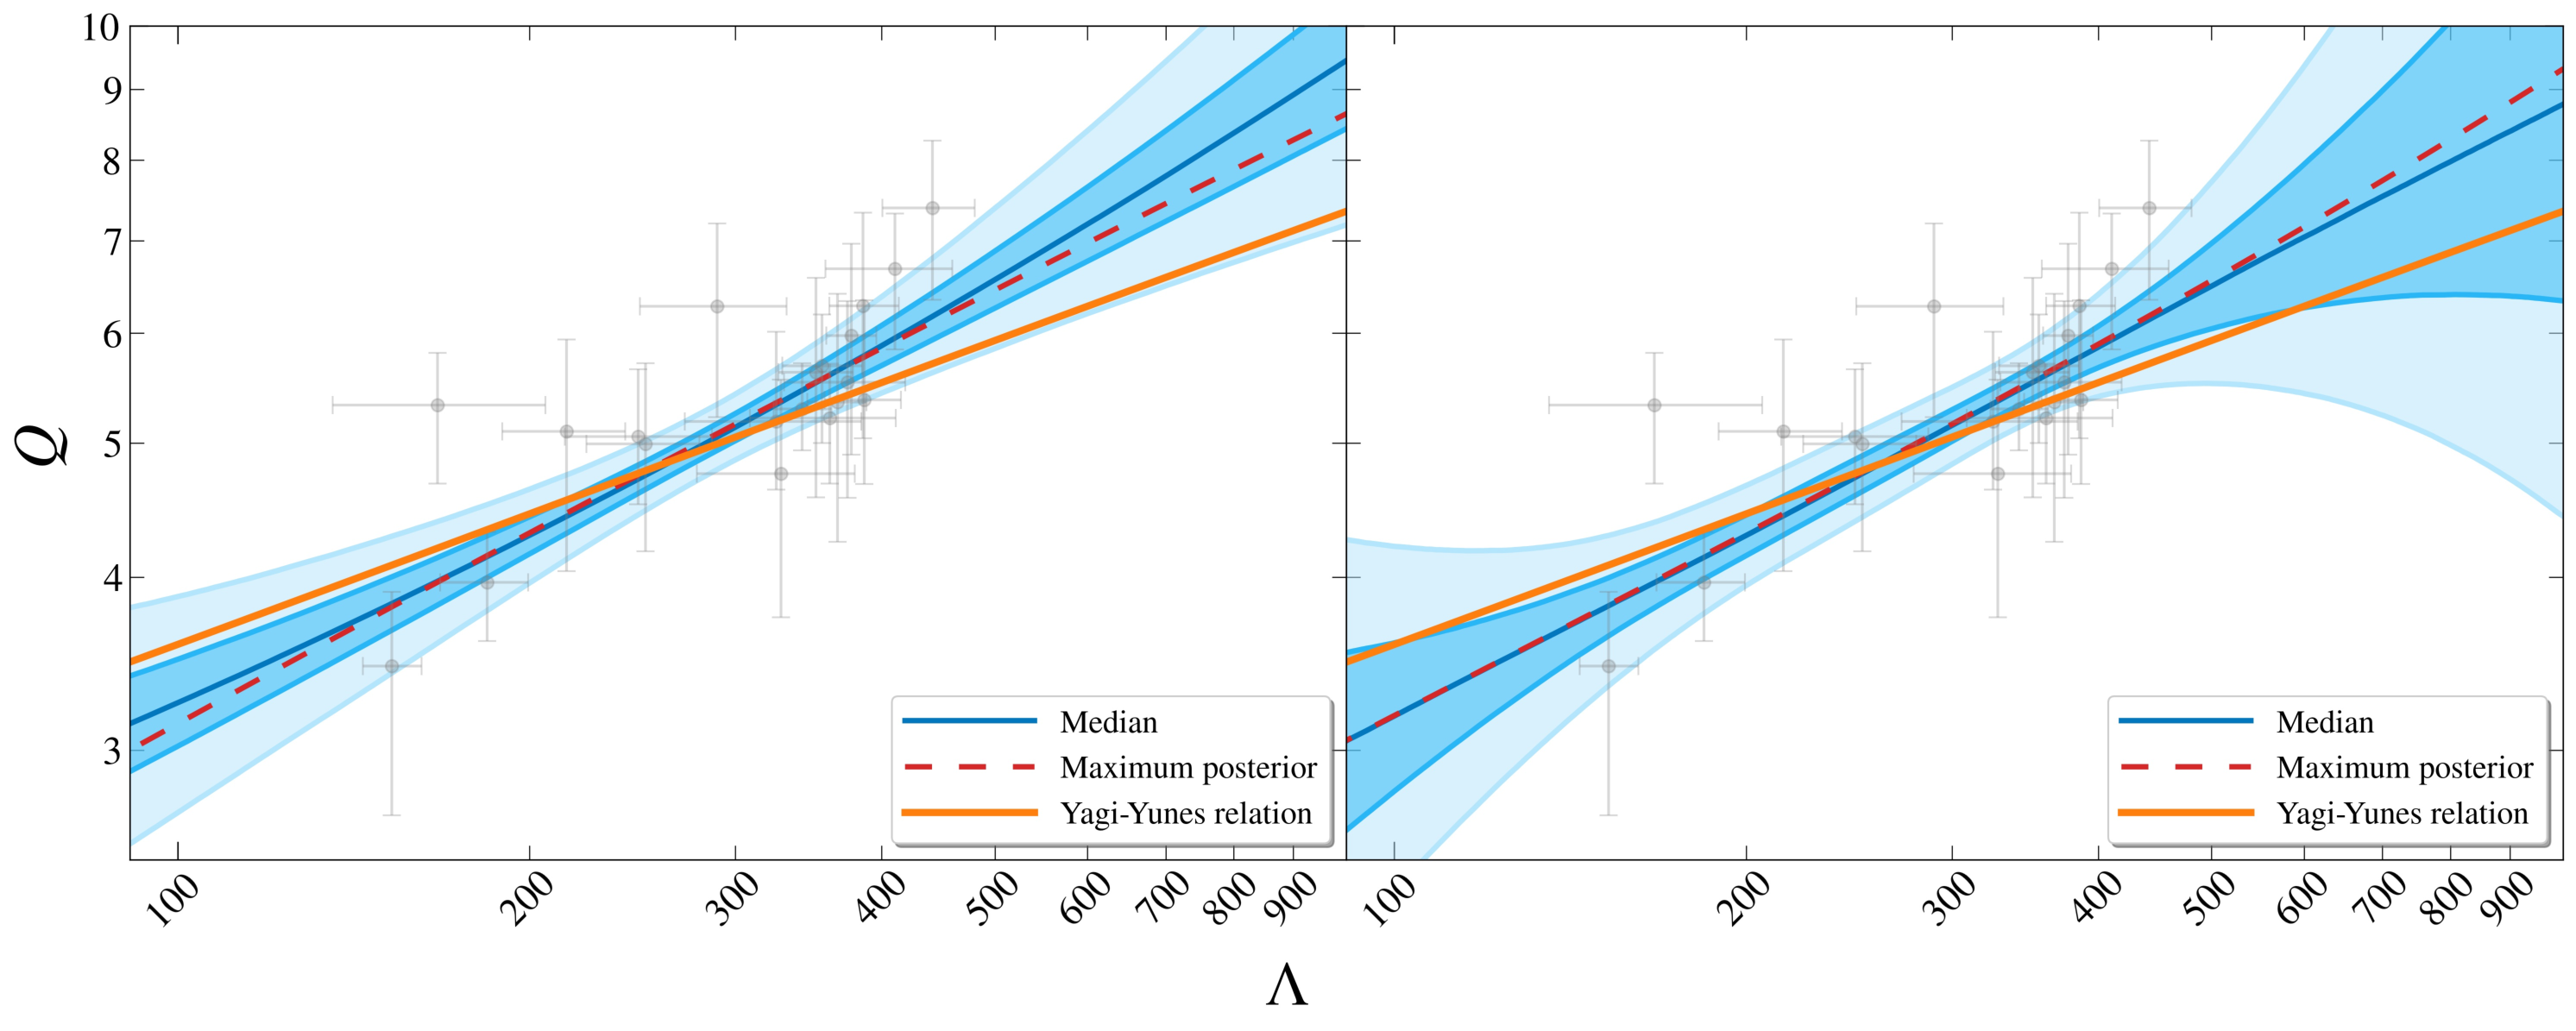
\includegraphics[width=\linewidth]{hierarchical_results_APR4_3d.pdf}
    \end{minipage}
    \caption{Similar to figure~\ref{5-d_Love_Q}, while for the quadratic and
    cubic polynomial models. Note that in the posterior, the orange lines
    indicate
    the reference values in table~\ref{prior_table}, while in the Love-Q
    panels, the orange lines indicate the original Yagi-Yunes Love-Q relation.
    \ZW{Therefore, I recommend to use different colors for these two kinds of
    ``true'' values, e.g., use black for the reference values in the posterior
    panels. (gray for the priors)}
    }\label{3-d_4-d_Love_Q}
\end{figure}
As shown in the previous two subsections, the observations from 20 simulated GW 
events can well constrain the two parameters in the linear model, while can not 
effectively constrain the five parameters in the quartic polynomial model. The two 
models are adopted in previous studies~\cite{Yagi:2013awa, Samajdar:2020xrd}, 
while here we further test the models in between them and see how the constraints 
change with the number of parameters. We perform the inference for the quadratic 
and cubic polynomial models, which contain three parameters $\{a_3, b_3, c_3\}$ 
and four parameters $\{a_4, b_4, c_4, d_4\}$, respectively. Similar to the linear 
model, the reference values of these parameters are obtained by directly fitting 
the Yagi-Yunes Love-Q relation and listed in table~\ref{prior_table}. The priors of the
hyperparameters keep the same as their counterparts in the quartic polynomial 
model, which are also listed in table~\ref{prior_table}.

We summarize the posterior distributions of the hyperparameters in the top row of 
figure~\ref{3-d_4-d_Love_Q}. In the quadratic model, strong degeneracy arises 
among the three parameters. The posterior of $b_3$ is almost the same as its 
prior. For $a_3$ and $c_3$, though the posteriors are narrower than the priors, 
their marginal distributions have very wide and flat peaks. In the cubic model, 
strong degeneracy still exists between $c_4$ and $d_4$, and the posterior of $b_4$ 
is also similar to its prior. Usually, posterior with large correlations and 
prior-like marginal distributions indicates redundant parameters in the model. 
Therefore, we conclude that the linear model is accurate enough in constraining 
the Love-Q relation with XG GW observations. This is consistent with the argument 
in Ref.~\cite{Samajdar:2020xrd} based on qualitative analysis, and in this work we present a quantitative demonstration. 

Same as before, we plot recovered Love-Q relations in the lower panels of 
figure~\ref{3-d_4-d_Love_Q}. We find the widths of the 90\% credible regions 
around $\Lambda \sim 400$ are similar for all the four models. While for
$\Lambda$ away from this region ($\Lambda \lesssim 200$ or $\Lambda \gtrsim 500$), 
the widths increase with the number of parameters. This may be the result of both 
the increased model complexity and the lack of data points in these
regions. 

%=============================
\section{Testing Modified Gravity: Dynamical Chern-Simons Gravity}
\label{sec:dCS}
%=============================

\begin{figure}[t]
    \centering
    \begin{minipage}{0.48\linewidth}
        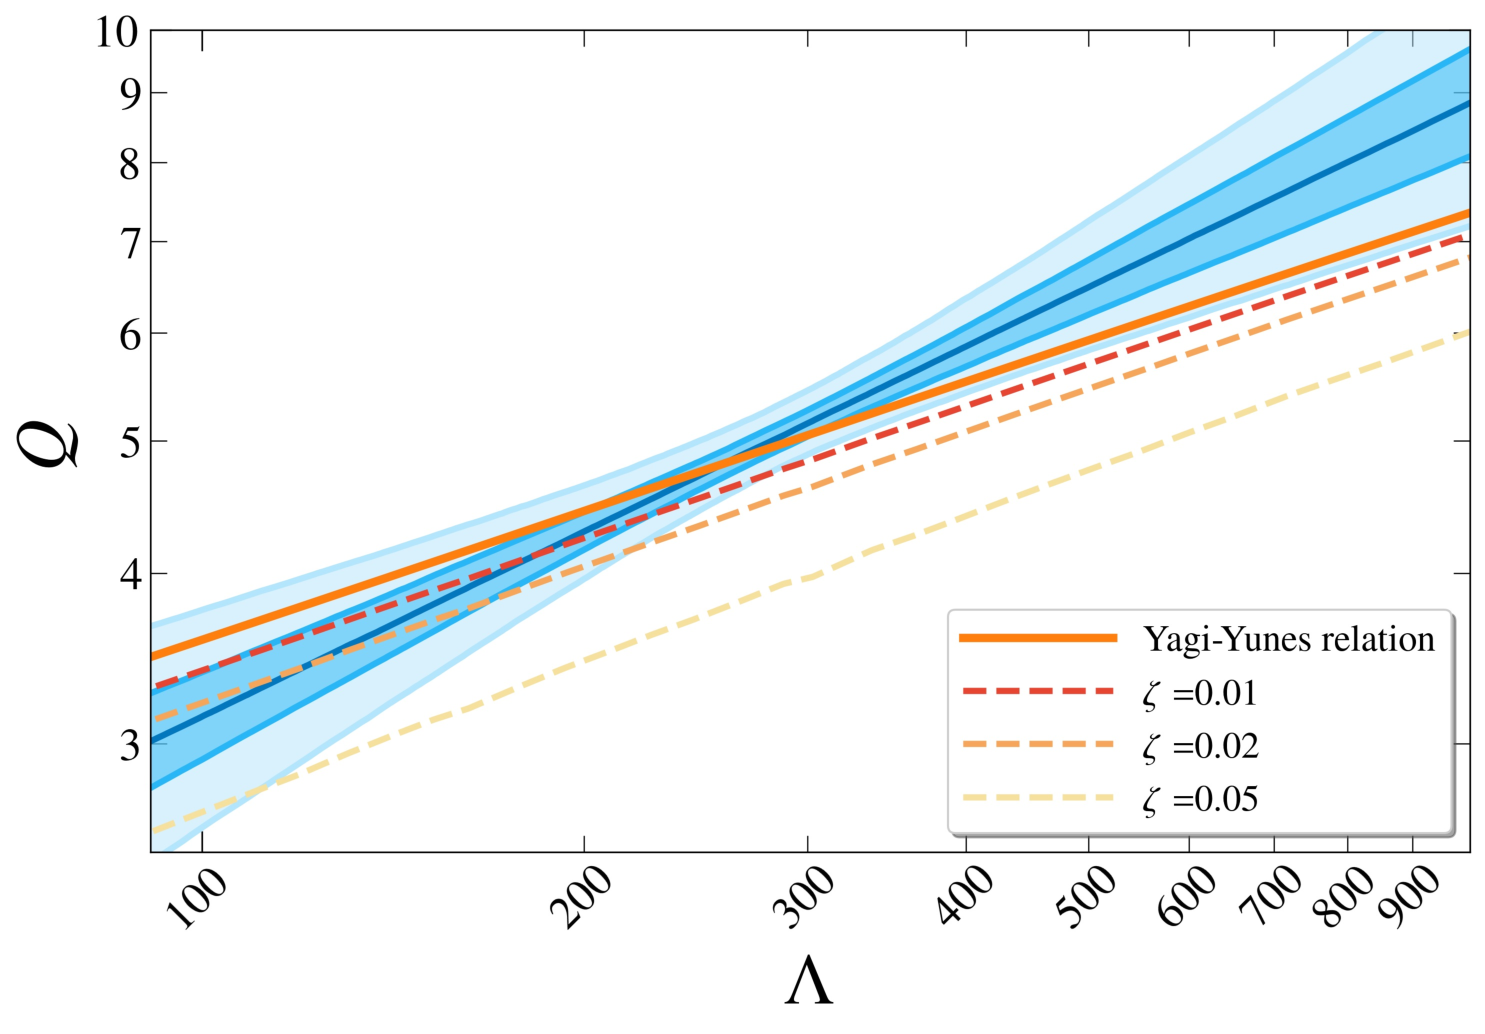
\includegraphics[width=\linewidth]{CS_zeta_APR4_2d.pdf}
    \end{minipage}
    \hfill
    \begin{minipage}{0.48\linewidth}
        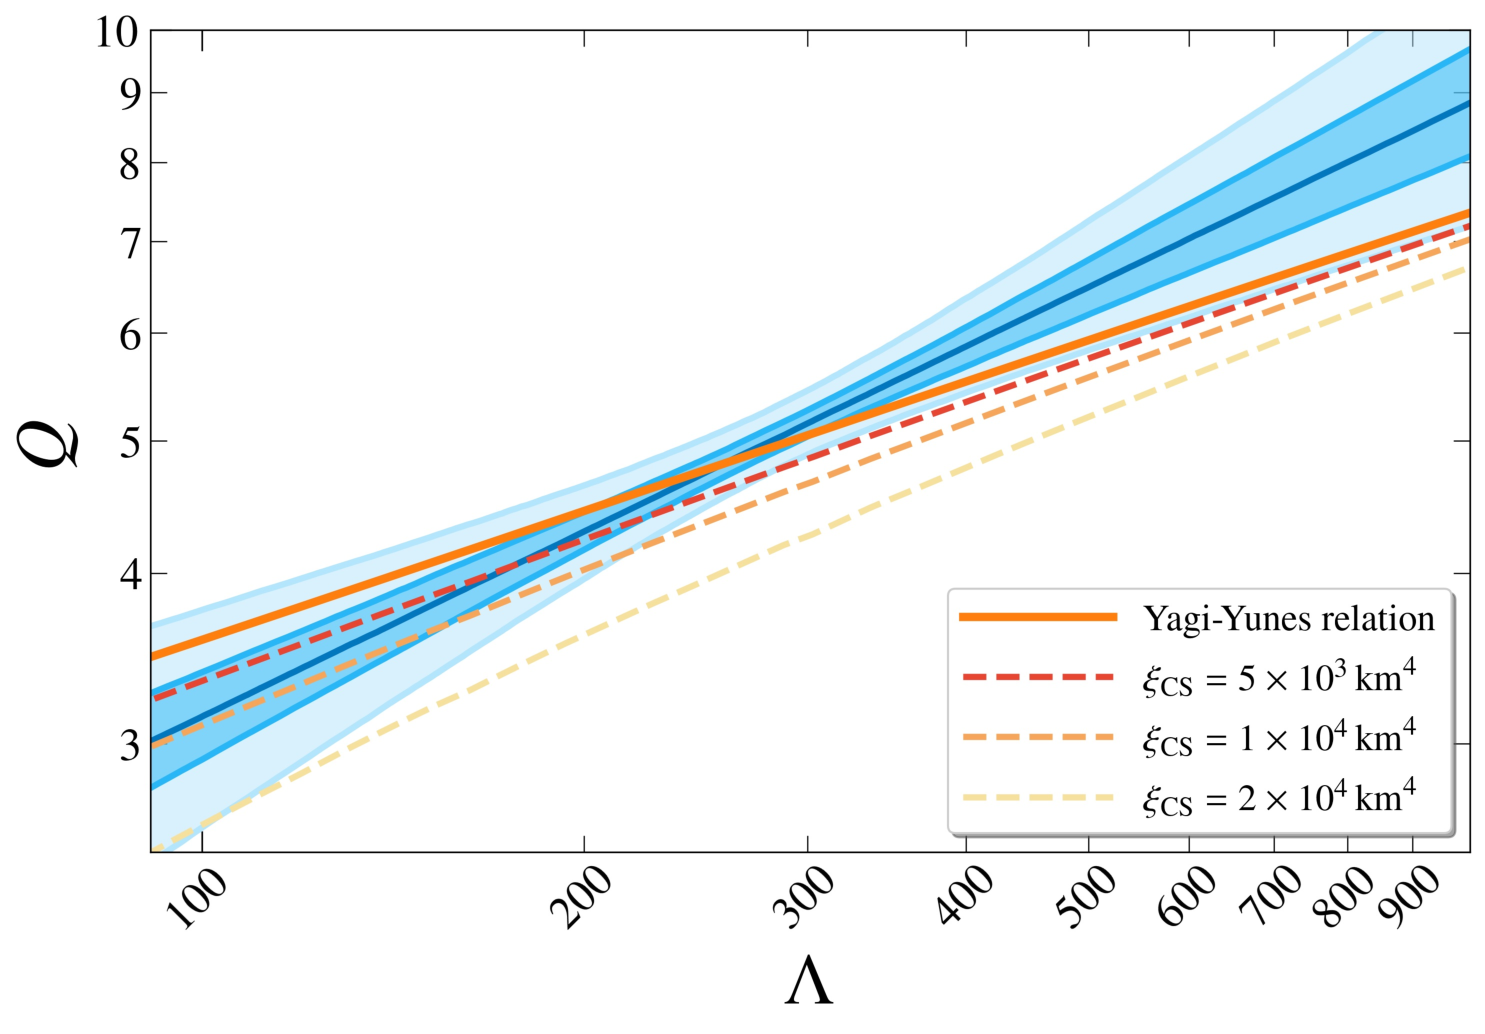
\includegraphics[width=\linewidth]{CS_xi_cs_APR4_2d.pdf}
    \end{minipage}
    \vspace{3mm}
    \begin{minipage}{0.48\linewidth}
        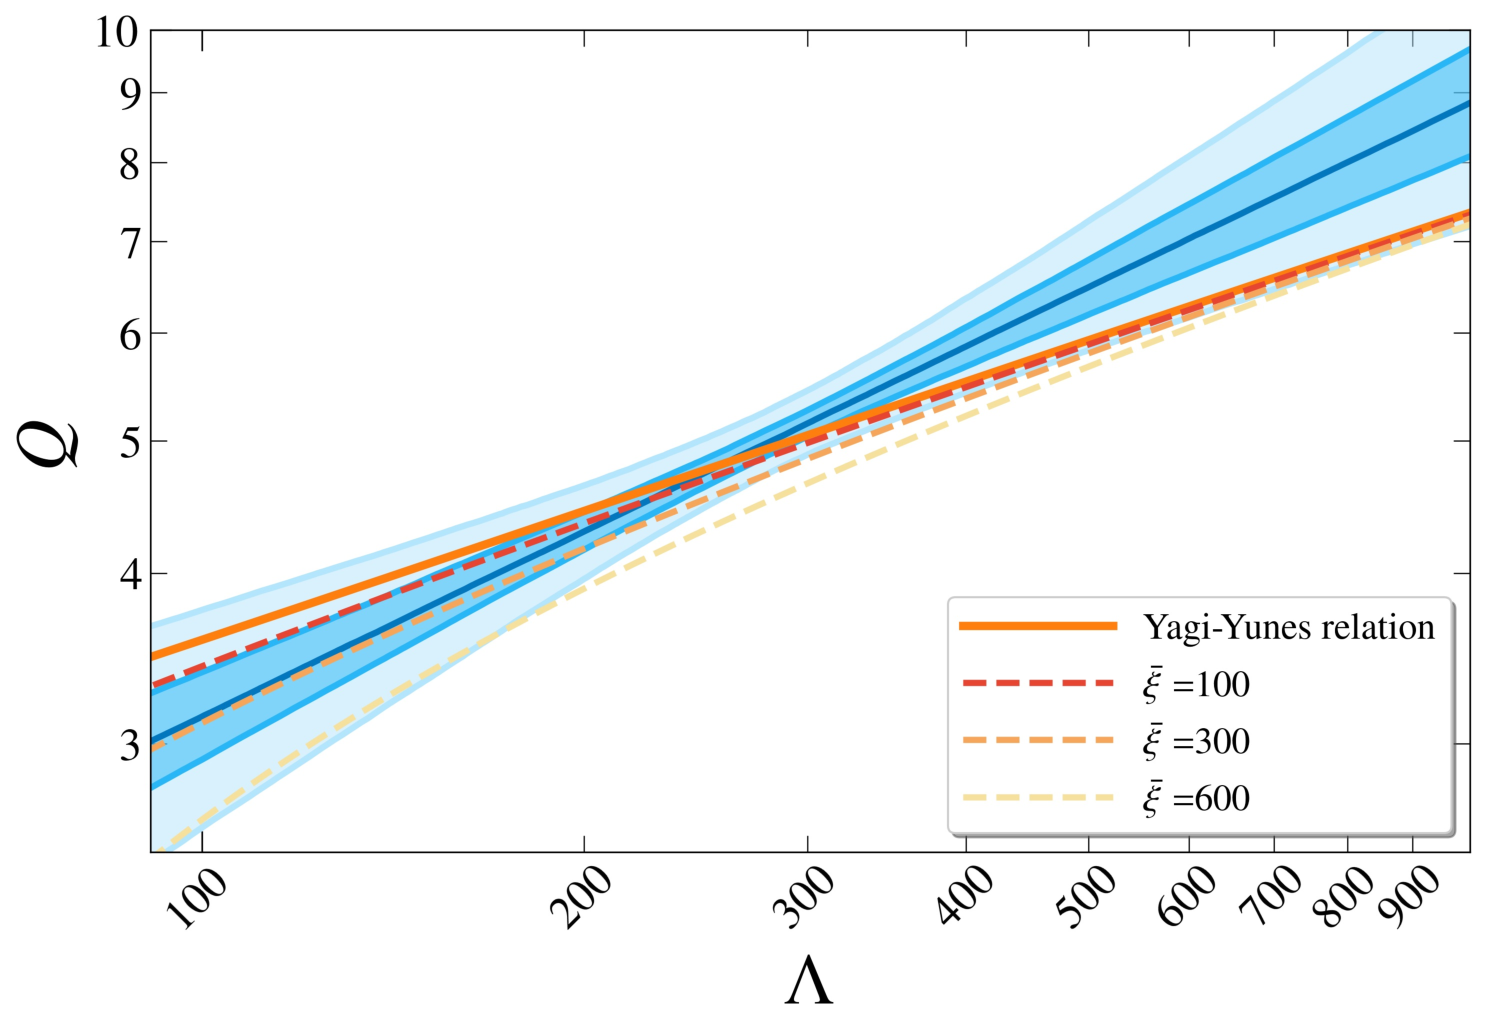
\includegraphics[width=\linewidth]{CS_xi_bar_APR4_2d.pdf}
    \end{minipage}
    \caption{Comparison of recovered Love-Q relation in GR
    and dCS predictions 
    with different coupling constants. Similar to figure~\ref{2-d_Love_Q}, the
    blue lines indicate the median of the recovered Love-Q relation, while the
    shaded regions represent the $50\%$ and $90\%$ credible intervals. For each of the coupling constants of 
    CS gravity $\zeta, \xi_{\mathrm{CS}}$ and $\bar\xi$, we take three values
    and plot corresponding Love-Q relations with APR4 EOS.\ZW{Still need to
    modified after the discussion in the main text.}}
    \label{cs_Love_Q}
\end{figure}
In this section, we investigate the potential of testing gravity theories with the 
inferred Love-Q relation from the GW observations. The I-Love-Q test can be 
powerful when significant difference in I-Love-Q relation between GR and modified 
gravity theories exists, for example, some parity-violating theories~\cite{Yagi_2017, Yunes:2025xwp}. 
Here we take the dynamical Chern-Simons (dCS) gravity~\cite{Jackiw:2003pm, Smith:2007jm,Alexander:2009tp} for discussion, 
which is well-motivated from heterotic superstring theory~\cite{Polchinski:1998rq,
Polchinski:1998rr}, loop quantum gravity~\cite{Alexander:2004xd,Taveras:2008yf,
Calcagni:2009xz} and effective field theories of inflation~\cite{Weinberg:2008hq}. 
The dCS gravity introduces parity violation and quadratic curvature terms into the action~\cite{Alexander:2009tp,Gupta:2017vsl}
\begin{equation}
   \label{cs_action}
   S = \int \mathrm{d}^4 x \sqrt{-g}\left[ \kappa_g \mathcal{R} + \frac{\alpha}{4} \mathcal{\vartheta} \mathcal{R}_{\nu\mu\rho\sigma} {}^{*}\mathcal{R}^{\mu\nu\rho\sigma} - \frac{\beta}{2}\nabla_{\mu}\mathcal{\vartheta}\nabla^{\mu}\mathcal{\vartheta} + \mathcal{L}_{\mathrm{mat}}\right]\,,
\end{equation}
where $g$ is the determinant of the metric, $\kappa_g= 1/16\pi$, $\mathcal{R}$ is 
the Ricci scalar, $\mathcal{R}_{\nu\mu\rho\sigma}$ and
$^{*}\mathcal{R}^{\mu\nu\rho\sigma}$ denote the Riemann tensor and its dual, 
$\mathcal{L}_{\mathrm{mat}}$ is the matter Lagrangian density, 
$\alpha$ and $\beta$ are the coupling constants in dCS gravity. We omit any 
potential for the pseudo-scalar field $\mathcal{\vartheta}$ in the action, 
following Ref.~\cite{Gupta:2017vsl}. $\mathcal{\vartheta}$ is taken to be 
dimensionless, and the quantity $\xi_{\mathrm{CS}}^{1/4} \equiv [\alpha^2/
(\kappa\beta)]^{1/4}$ can be explained as 
the characteristic length of dCS gravity~\cite{Yunes:2009hc,Yagi:2012ya}. 

%\ZW{Maybe you need to re-introduce the parameters in the Love-Q relation and the relation between them and the coupling constant in dCS gravity.}
The dCS gravity predicts Love-Q relations that are degenerate with the one in GR 
only when the coupling constants approach zero~\cite{Yagi:2013bca,
Yagi:2013awa,Gupta:2017vsl}. The characteristic length has been constrained by 
current Solar System observations to $\xi_{\mathrm{CS}}^{1/4}<\mathcal{O}(10^8)$~km~\cite{Ali-Haimoud:2011zme,Yagi:2012ya}. 
For a Love-Q test, Ref.~\cite{Yagi:2013mbt} obtained the dCS correction to the NS 
quadrupole moment and Ref.~\cite{Yagi:2011xp} indicates that the tidal 
deformability is the same as the one in GR at leading order in small coupling 
approximation $\zeta \equiv \xi_{\mathrm{CS}} M^2/R^6 \ll 1$, regarding the dCS 
gravity as an effective theory. Refs.~\cite{Yagi_2017,Yagi:2013mbt,Gupta:2017vsl} 
have discussed the Love-Q relation under dCS gravity and find that the relation 
becomes EOS-sensative with $\xi_{\mathrm{CS}}$ or $\zeta$ fixed. However, but with 
$\bar{\xi}\equiv \xi_{\mathrm{CS}}/M^4$ fixed, the Love-Q relation remains 
universal and the EOS variation is of $\mathcal{O}(1\%)$. Ref.~\cite{Gupta:2017vsl} 
parameterized the relation between the dCS correction to $Q$ (denoted as $Q_{\mathrm{CS}}$) and the tidal deformability $\Lambda$ as follows
\begin{equation}
    \label{cs_Love_Q_eq}
    \ln (Q_{\mathrm{CS}}/\bar{\xi}) = a + b \ln \Lambda + c \ln^{2} \Lambda
\end{equation} 
where the fitting coefficients $a=-3.443, b=-0.550$ and $c=-0.023$. 

Following Ref.~\cite{Yagi_2017}, we calculate the dCS Love-Q relation with $\zeta, \xi_{\mathrm{CS}}$ and $\bar{\xi}$ 
fixed respectively assuming the APR4 EOS, which has been assumed in our simulation 
in section~\ref{sec:simulation}. The results are demonstrated in figure~\ref{cs_Love_Q}. 
We compare the hierarchical Bayesian inference constraint of the Love-Q relation 
using the linear model (figure~\ref{2-d_Love_Q}) with some possible Love-Q 
relations with respect to certain coupling constants in dCS gravity. From 
figure~\ref{cs_Love_Q} we can conclude that our Love-Q test of dCS gravity can 
constrain the characteristic length $\xi_{\mathrm{CS}}^{1/4} \lesssim \mathcal{O}(10^1)$~km, 
which is in agreement with the results given by Refs.~\cite{Yagi:2013bca,Yagi:2013awa}. 
For the other two coupling constants, our inference results place constraints of 
$\zeta \lesssim \mathcal{O}(10^{-2})$ and $\bar{\xi} \lesssim \mathcal{O}(10^{3})$.

%=============================
\section{Conclusion}
\label{sec:conclusion}
%=============================

In this work, we investigate the prospects of inferring the Love-Q relation of NSs
with future ground based GW observations.
Extending the inference procedure in
Ref.~\cite{Samajdar:2020xrd}, 
We adopt the hierarchical Bayesian framework to effectively combine the
information from multiple GW events, extending the linear fitting model in
previous works~\cite{Samajdar:2020xrd}. The hierarchical Bayesian framework
separate the inferences into two steps, the auxiliary single-event
inference and the hyperparameter inference, which avoids a direct high-dimensional
inference for all the parameters simultaneously while still takes into account
degeneracy and non-Gaussianity in the single-event parameters. We also discuss
the impact of the event number on the constraints, and find that the loudest 10 events
dominate the information in constraining the Love-Q relation. Similar phenomena
were also found in studies of constraining the EOSs with GW observations~\cite{Lackey:2014fwa,Landry:2020vaw,Pang:2020ilf,Finstad:2022oni,Bandopadhyay:2024zrr,Wang:2024xon}.

We are the first to conduct a systematic study on different parameterization models
when inferring the Love-Q relation with GWs. Considering the quartic polynomial
model proposed by \citet{Yagi:2013awa} and the linear model adopted by
\citet{Samajdar:2020xrd} as two extremes, we conduct the inference with
four polynomial models
from linear to quartic terms respectively. As shown in
section~\ref{sec:results}, we quantitatively demonstrate that
the linear model is accurate enough to describe the Love-Q relation in the
inference. Also, as the number of parameters increases, more significant
degeneracy or poorly constrained parameters appear in the posteriors, while the recovered Love-Q relations keep similar in the region where most data points gather.

We also test the potential of using the inferred Love-Q relation to
constrain modified gravity theories in Section~\ref{sec:dCS}.
Taking the dCS gravity as an example, we find that the inferred Love-Q relation
can place a constraint on the dCS characteristic length about
$\xi_{\mathrm{CS}}^{1/4} \lesssim \mathcal{O}(10^1)$~km, which is seven orders
of magnitude tighter than that from current Solar System
observations~\cite{Ali-Haimoud:2011zme,Yagi:2012ya}, and consistent with
previous predictions~\cite{Yagi:2013bca,Yagi:2013awa}. This highlights the power
of inferring the Love-Q relation from GWs in testing gravity theories. \ZW{Plz
check the parameters to be constrained and corresponding limits.}

There are several extensions to this work. Firstly, we assume the aligned-spin BNS systems, while
realistic BNS systems may have spin precession, which leads to additional
biases or uncertainties~\cite{Williamson:2017evr}. The waveform modelling can
also have similar issues~\cite{Purrer:2019jcp,Gamba:2020wgg}. 
Also, in the XG era, the GW signals are possibly overlapping with each
other, complicating the data analysis~\cite{Pizzati:2021apa, Samajdar:2021egv,
Wang:2023ldq, Johnson:2024foj, Wang:2025ckw}.
Moreover, the Yagi-Yunes universal relations were originally found and discussed
for a single NS. For BNS systems, these universal relations may hold when the
two NSs have similar masses, but still require careful
inspection~\cite{Shao:2022koz, Saffer:2021gak}. Additionally, the octupole or
higher-order multipole moments of NSs also contribute to the GW waveform and can
be universally related to the quadrupole moment~\cite{Yagi_2017,Abac:2023ujg}.
We leave the exploration of simultaneous or independent inference of more
universal relations to future works.

%=============================
\acknowledgments

\clearpage

\bibliographystyle{apsrev4-1}
% \bibliographystyle{unsrt}
\bibliography{HBAGW_jcap}
\end{document}
